\documentclass[12pt,letterpaper,oneside]{book}
\usepackage{../afitStyleFiles/afitThesis}
\usepackage{../afitStyleFiles/sf298}
\usepackage[pdftex,pdfpagelabels,bookmarks,hyperindex,hyperfigures]{hyperref}
\usepackage[nogroupskip,automake,nonumberlist,nopostdot,shortcuts,section]{glossaries}

\mathchardef\mhyphen="2D % Define a "math hyphen"
\graphicspath{{../Figures/}}
\makeglossaries
\newacronym{AFP}{AFP}{Adaptive Failure Prediction}
\newacronym{OFP}{OFP}{Online Failure Prediction}
\newacronym{CPU}{CPU}{Central Processing Unit}
\newacronym{G-SWFIT}{G-SWFIT}{Generic Software Fault Injection Technique}
\newacronym{W-SWFIT}{W-SWFIT}{Windows Software Fault Injection Tool}
\newacronym{CSCS}{CSCS}{Cyber Security and Control System}
\newacronym{NOS}{NOS}{Network Operation Squadrons}
\newacronym{DOD}{DOD}{Department of Defense}
\newacronym{GHSMM}{GHSMM}{Generalized Hidden Semi-Markov Model}
\newacronym{SVM}{SVM}{Support Vector Machine}
\newacronym{IP}{IP}{Internet Protocol}
\newacronym{CRISP-DM}{CRISP-DM}{Cross Industry Standard Process for Data Mining}
\newacronym{ROC}{ROC}{Receiver Operating Characteristic}
\newacronym{MS}{MS}{Microsoft}
\newacronym{AD}{AD}{Active Directory}
\newacronym{GB}{GB}{Gigabyte}
\newacronym{GHz}{GHz}{Gigahertz}
\newacronym{VM}{VM}{Virtual Machine}
\newacronym{PFM}{PFM}{Proactive Fault Management}
\newacronym{DC}{DC}{Domain Controller}
\newacronym{ASLR}{ASLR}{Address Space Layout Randomization}
\newacronym{DNS}{DNS}{Domain Name System}
\newacronym{D-PLG}{D-PLG}{Distributed PowerShell Load Generator}
\newacronym{RDP}{RDP}{Remote Desktop Protocol}
\newacronym{SQL}{SQL}{Structured Query Language}
\newacronym{API}{API}{Application Programming Interface}
\newacronym{TP}{TP}{True Positive}
\newacronym{FP}{FP}{False Positive}
\newacronym{TN}{TN}{True Negative}
\newacronym{FN}{FN}{False Negative}
\newacronym{FPR}{FPR}{False Positive Rate}
\newacronym{TPR}{TPR}{True Positive Rate}
\newacronym{NPV}{NPV}{Negative Predictive Value}
\newacronym{AUC}{AUC}{Area Under the Curve}
\newacronym{IIS}{IIS}{Internet Information Service}
\newacronym{ODC}{ODC}{Orthogonal Defect Classification}
\newacronym{ANN}{ANN}{Artificial Neural Network}
\newacronym{NN}{NN}{Neural Network}
\newacronym{RNN}{RNN}{Recurrent Neural Network}
\newacronym{LSTM}{LSTM}{Long Short-Term Memory}


\input{Preamble/titlepage}
%% myFigures.tex
% A common file to store all figure definitions
%
% In preparing your thesis, one of the first things you should do is
% organize your figures.  Then, one of the last things you'll do is
% reorder your figures so they display where you want them to in the
% text.  Organizing figure definitions in a common files helps:
%
%   1. Write new figures using earlier examples.
%
%   2.  Isolate code and minimize the risk of introducing bugs in the
%   final editing process.  Trust me, moving around just one line of
%   code is easier.
%
%   3.  Reuse figures in other papers.  <=== the best reason!
%
% Note command names can not include numbers and special characters.
%
% To make the file more searchable, use naming conventions that map
% the graphics filename labSetup.jpg to the command name \figlabSetup to the
% figure label fig:labSetup.
% 

\newcommand{\figproactiveFaultManagement}[1]{\begin{figure}
 \begin{center}
    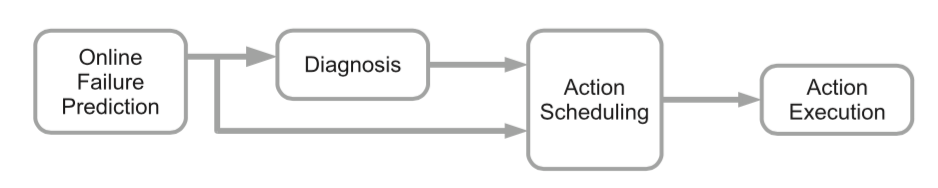
\includegraphics[width=#1]{proactiveFaultManagement}
     \caption[Proactive Fault Management~\cite{salfnerSurvey}]{The stages of
     proactive fault management~\cite{salfnerSurvey}.}
     \label{fig:proactiveFaultManagement}
 \end{center}
\end{figure}
}

\newcommand{\figonlinePrediction}[1]{\begin{figure}
 \begin{center}
    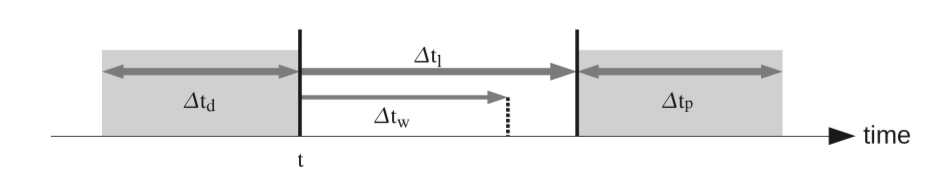
\includegraphics[width=#1]{onlinePrediction}
     \caption[\ac{OFP}~\cite{salfnerSurvey}]{The timeline for
     \ac{OFP}~\cite{salfnerSurvey}.}
     \label{fig:onlinePrediction}
 \end{center}
\end{figure}
}

\newcommand{\figfailureFlowDiagram}[1]{\begin{figure}
 \begin{center}
    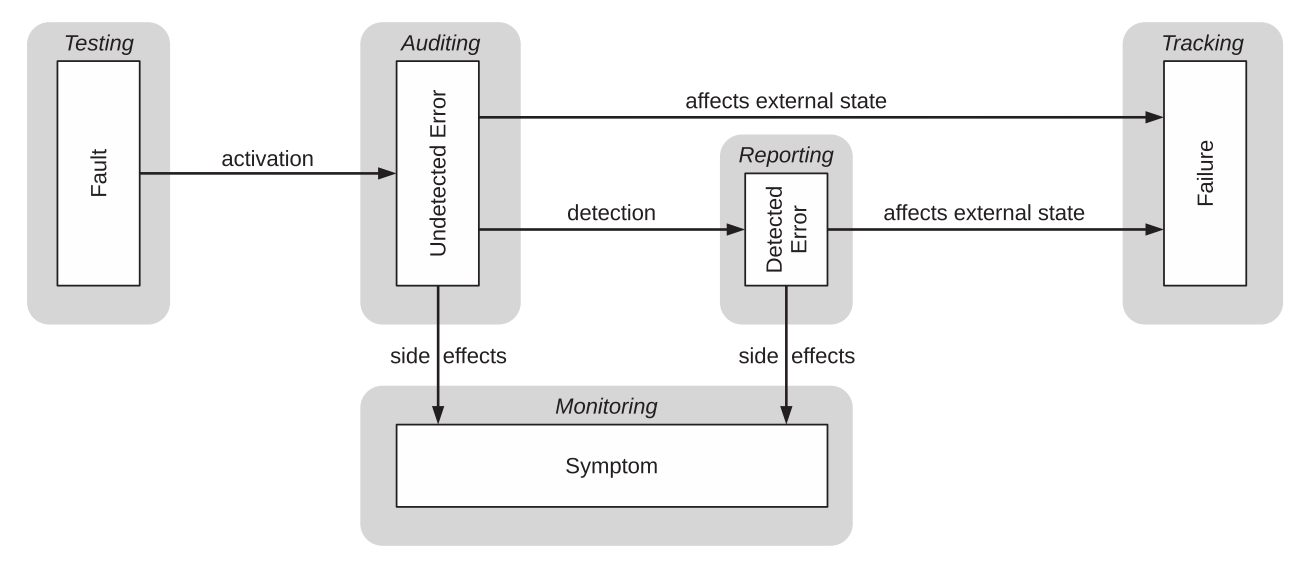
\includegraphics[width=#1]{failureFlowDiagram}
     \caption[Failure Flow Diagram~\cite{salfnerSurvey}]{How faults and errors
     evolve into failure with the associated methods for detection represented
     by enclosing gray boxes~\cite{salfnerSurvey}.}
     \label{fig:failureFlowDiagram}
 \end{center}
 %\vspace{-0.2 in}
\end{figure}
}

\newcommand{\figROC}[1]{\begin{figure}
 \begin{center}
    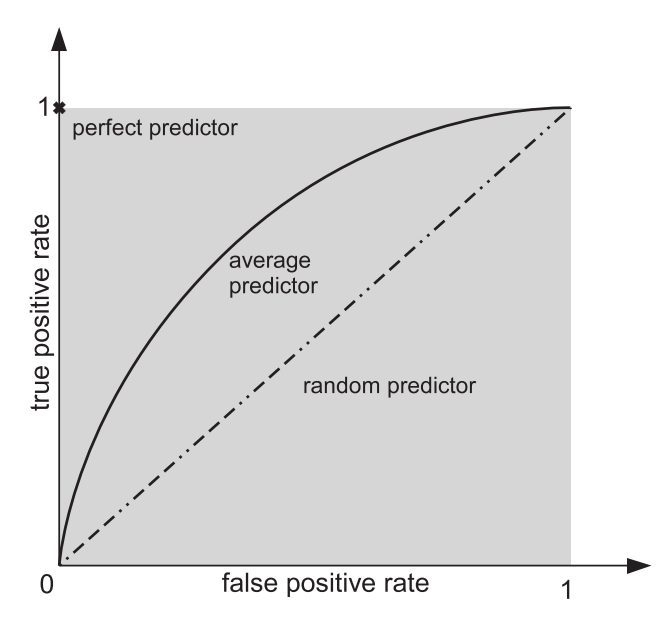
\includegraphics[width=#1]{ROC}
     \caption[Sample \ac{ROC} Plots~\cite{salfnerSurvey}]{\ac{ROC} plots of
     perfect, average, and random predictors~\cite{salfnerSurvey}.}
     \label{fig:ROC}
 \end{center}
\end{figure}
}

\newcommand{\figprecisionRecallCurve}[1]{\begin{figure}
 \begin{center}
    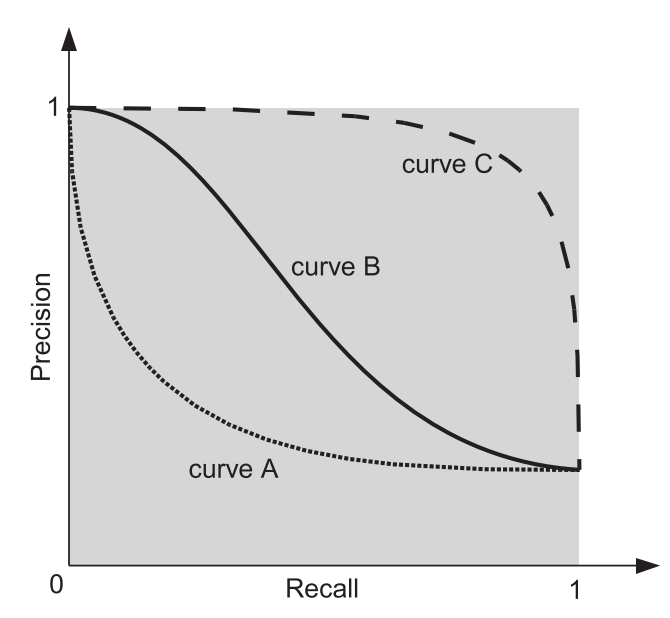
\includegraphics[width=#1]{precisionRecallCurve}
     \caption[Sample Precision/Recall Curves~\cite{salfnerSurvey}]{Sample
     precision/recall curves~\cite{salfnerSurvey}.  Curve $A$ represents a
     poorly performing predictor, curve $B$ an average predictor, and curve $C$
     an exceptional predictor.}
     \label{fig:precisionRecallCurve}
 \end{center}
\end{figure}
}

\newcommand{\figpatternRecognition}[1]{\begin{figure}
 \begin{center}
    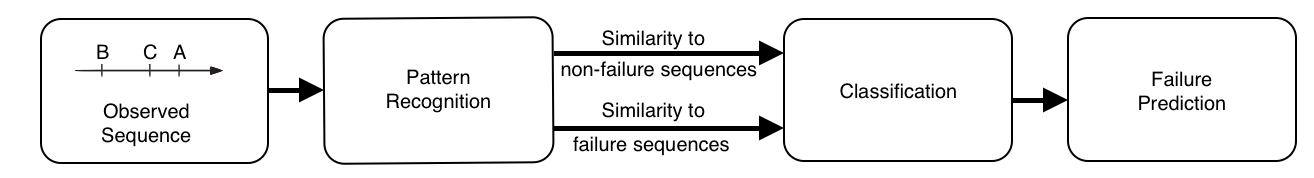
\includegraphics[width=#1]{patternRecognition}
     \caption[Pattern recognition in reported errors~\cite{salfnerSurvey}]{How
     pattern recognition is accomplished in reported
     errors~\cite{salfnerSurvey}.}
     \label{fig:patternRecognition}
 \end{center}
\end{figure}
}

\newcommand{\figAFP}[1]{\begin{figure}[t!h]
 \begin{center}
    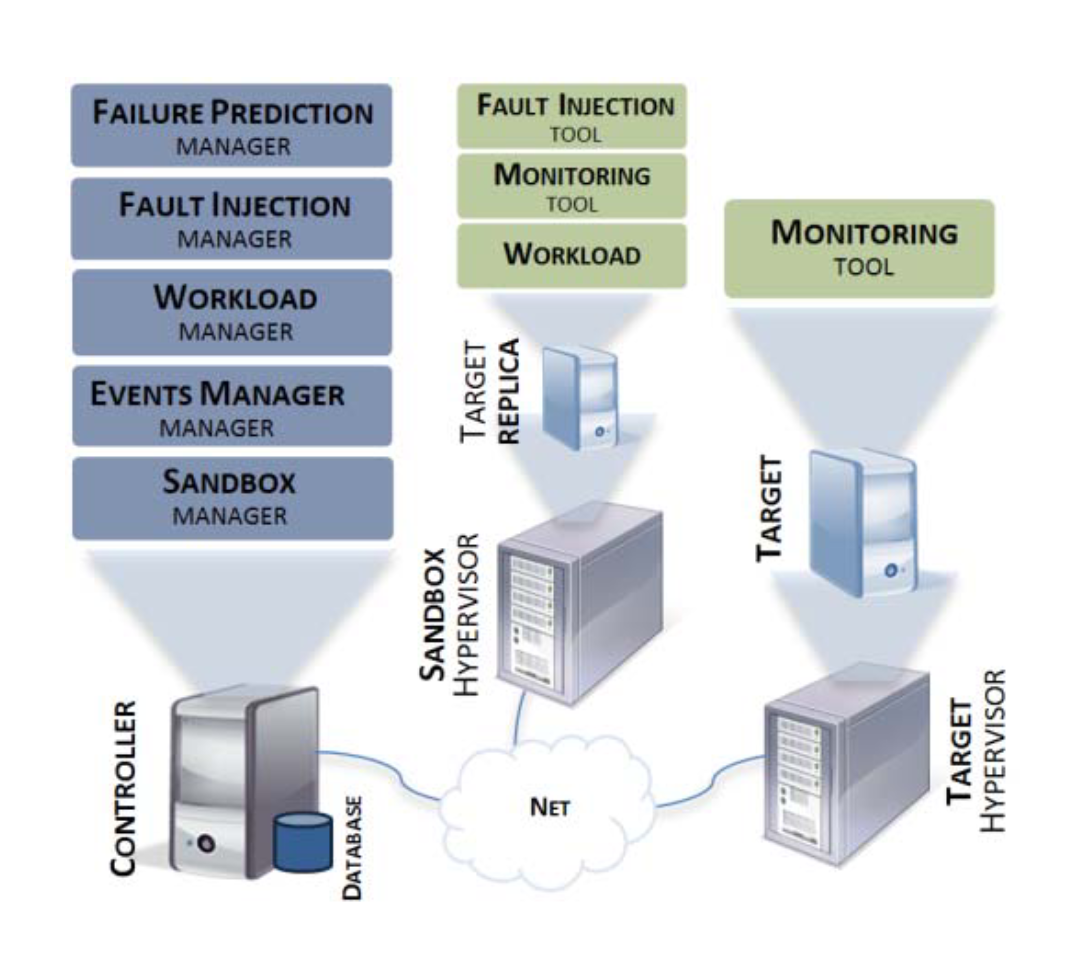
\includegraphics[width=#1]{AFP}
     \caption{The \ac{AFP} framework~\cite{irrera2015}.}
     \label{fig:AFP}
 \end{center}
\end{figure}
}

\definecolor{airforceblue}{rgb}{0.36, 0.54, 0.66}
\definecolor{armygreen}{rgb}{0.29, 0.33, 0.13}

\newcommand{\figannotatedAFPcolor}{\begin{figure}
 \begin{center}
     \begin{overpic}[width=5in,scale=.25]{annotatedAFPcolor}
       \put(8,0){
         \begin{tikzpicture}
           [node font=\footnotesize, label/.style={rectangle, draw,
           fill=airforceblue, text width=2cm, text badly centered, minimum
           height=0.5cm, rounded corners}]

           \node[label] (FPMgr)
             {\textcolor{white}{\ref{sec:failurePrediction}}};
           \node[label, below=1.2cm of FPMgr] (FIMgr) 
             {\textcolor{white}{\ref{sec:faultInjectionMgr}}};
           \node[label, below=1.3cm of FIMgr] (WMgr) 
             {\textcolor{white}{\ref{sec:workloadMgr}}};
           \node[label, below=1.2cm of WMgr] (EMMgr) 
             {\textcolor{white}{\ref{sec:eventsManagerMgr}}};
           \node[label, below=1.2cm of EMMgr] (SMgr) 
             {\textcolor{white}{\ref{sec:sandboxMgr}}};
           \node[label, below=4.75cm of SMgr] (Controller) 
             {\textcolor{white}{\ref{sec:controller}}};
         \end{tikzpicture}
       }

       \put(40,60.5){
         \begin{tikzpicture}
           [node font=\footnotesize, label/.style={rectangle, draw,
           fill=armygreen, text width=2cm, text badly centered, minimum
           height=0.5cm, rounded corners}]

           \node[label] (Sandbox)
             {\textcolor{white}{\ref{sec:sandbox}}};
           \node[label, below=1.2cm of Sandbox] (SBFITool)
             {\textcolor{white}{\ref{sec:faultInjectionTool}}};
           \node[label, below=0.95cm of SBFITool] (SBMTool) 
             {\textcolor{white}{\ref{sec:sandboxMonitoringTool}}};
           \node[label, below=0.95cm of SBMTool] (SBWorkload) 
             {\textcolor{white}{\ref{sec:sandboxWorkload}}};
         \end{tikzpicture}
       }

       \put(66,0){
         \begin{tikzpicture}
           [node font=\footnotesize, label/.style={rectangle, draw,
           fill=armygreen, text width=2cm, text badly centered, minimum
           height=0.5cm, rounded corners}]

           \node[label] (MonTool)
             {\textcolor{white}{\ref{sec:targetMonitoringTool}}};
           \node[label, below=7.85cm of MonTool] (Target)
             {\textcolor{white}{\ref{sec:target}}};
         \end{tikzpicture}
       }
     \end{overpic}
     \caption[Annotated \ac{AFP} Framework~\cite{irrera2015}]{The \ac{AFP}
     framework implementation~\cite{irrera2015} with modified components
     highlighted.}
     \label{fig:annotatedAFP}
 \end{center}
\end{figure}
}

\newcommand{\figannotatedAFP}{\begin{figure}
 \begin{center}
     \begin{overpic}[width=5in,scale=.25]{annotatedAFP}
       \put(8,0){
         \begin{tikzpicture}
           [node font=\footnotesize, label/.style={rectangle, draw,
           fill=white, text width=2cm, text badly centered, minimum
           height=0.5cm, rounded corners}]

           \node[label] (FPMgr)
             {\textcolor{black}{\ref{sec:failurePrediction}}};
           \node[label, below=1.2cm of FPMgr] (FIMgr) 
             {\textcolor{black}{\ref{sec:faultInjectionMgr}}};
           \node[label, below=1.3cm of FIMgr] (WMgr) 
             {\textcolor{black}{\ref{sec:workloadMgr}}};
           \node[label, below=1.2cm of WMgr] (EMMgr) 
             {\textcolor{black}{\ref{sec:eventsManagerMgr}}};
           \node[label, below=1.2cm of EMMgr] (SMgr) 
             {\textcolor{black}{\ref{sec:sandboxMgr}}};
           \node[label, below=4.75cm of SMgr] (Controller) 
             {\textcolor{black}{\ref{sec:controller}}};
         \end{tikzpicture}
       }

       \put(40,60.5){
         \begin{tikzpicture}
           [node font=\footnotesize, label/.style={rectangle, draw,
           fill=white, text width=2cm, text badly centered, minimum
           height=0.5cm, rounded corners}]

           \node[label] (Sandbox)
             {\textcolor{black}{\ref{sec:sandbox}}};
           \node[label, below=1.2cm of Sandbox] (SBFITool)
             {\textcolor{black}{\ref{sec:faultInjectionTool}}};
           \node[label, below=0.95cm of SBFITool] (SBMTool) 
             {\textcolor{black}{\ref{sec:sandboxMonitoringTool}}};
           \node[label, below=0.95cm of SBMTool] (SBWorkload) 
             {\textcolor{black}{\ref{sec:sandboxWorkload}}};
         \end{tikzpicture}
       }

       \put(66,0){
         \begin{tikzpicture}
           [node font=\footnotesize, label/.style={rectangle, draw,
           fill=white, text width=2cm, text badly centered, minimum
           height=0.5cm, rounded corners}]

           \node[label] (MonTool)
             {\textcolor{black}{\ref{sec:targetMonitoringTool}}};
           \node[label, below=7.85cm of MonTool] (Target)
             {\textcolor{black}{\ref{sec:target}}};
         \end{tikzpicture}
       }
     \end{overpic}
     \caption[Annotated \ac{AFP} Framework~\cite{irrera2015}]{The \ac{AFP}
     framework implementation~\cite{irrera2015} with modified components
     highlighted.}
     \label{fig:annotatedAFP}
 \end{center}
\end{figure}
}

\newcommand{\figTrainingPhase}[1]{\begin{figure}[h!t]
 \begin{center}
  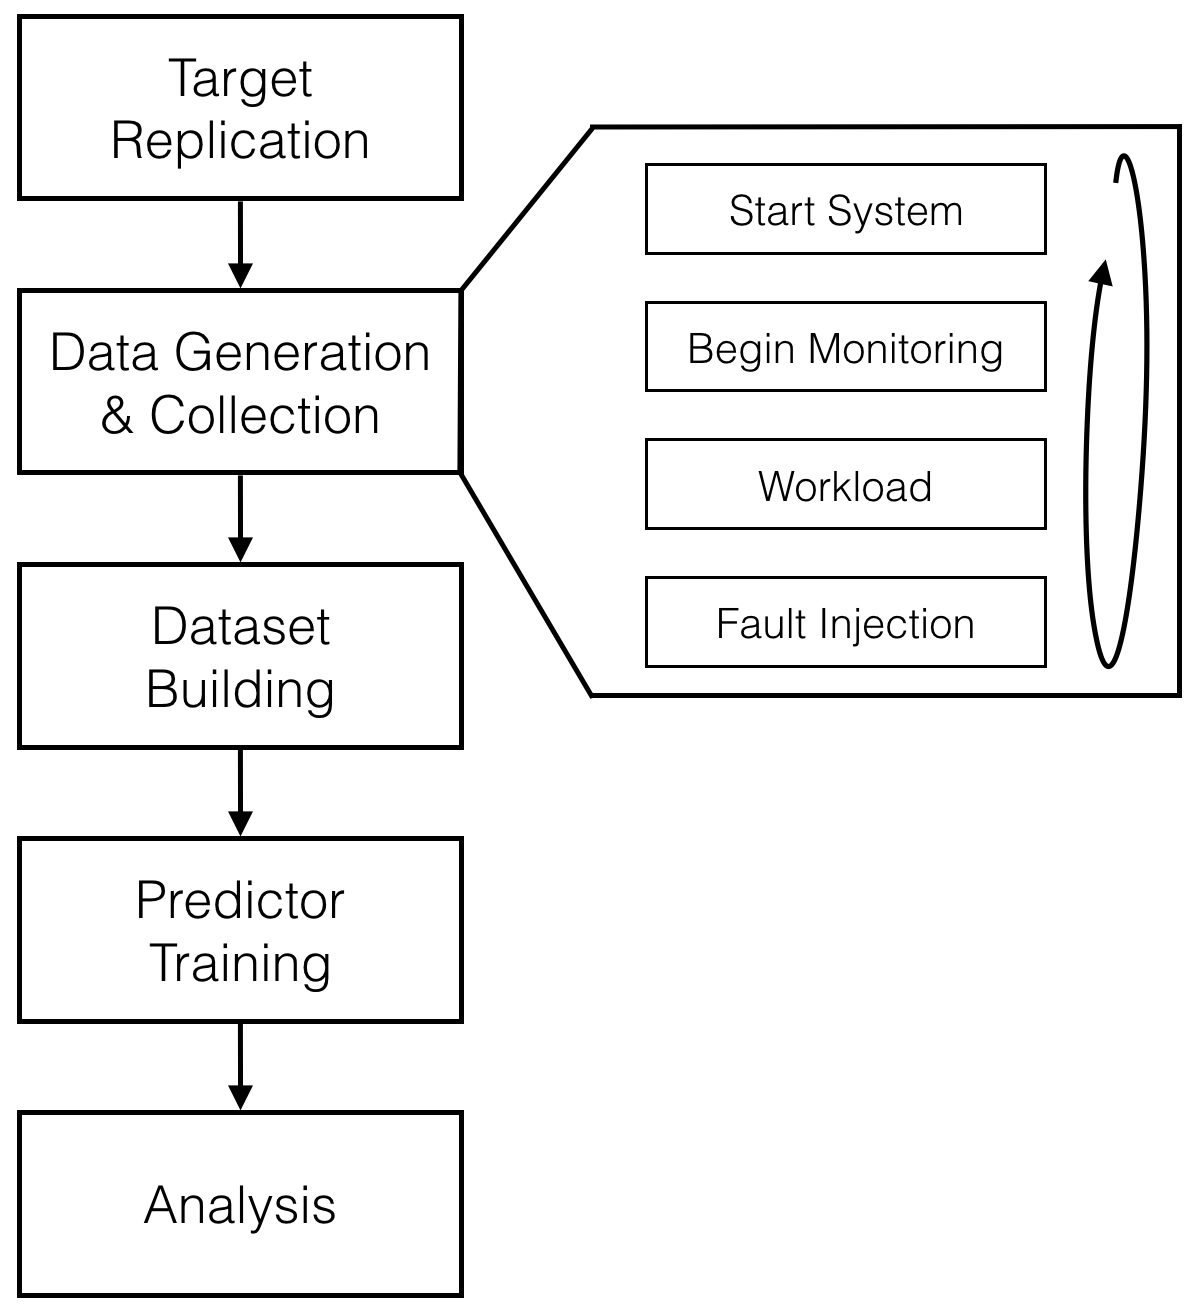
\includegraphics[width=#1]{TrainingPhase}
  \caption[\ac{AFP} Training Phase~\cite{irrera2015}]{The flow of the major
  steps involved in the \ac{AFP} framework training phase~\cite{irrera2015}.}
  \label{fig:TrainingPhase}
 \end{center}
\end{figure}
}

\newcommand{\figExecutionPhase}[1]{\begin{figure}[h!t]
  \begin{center}
    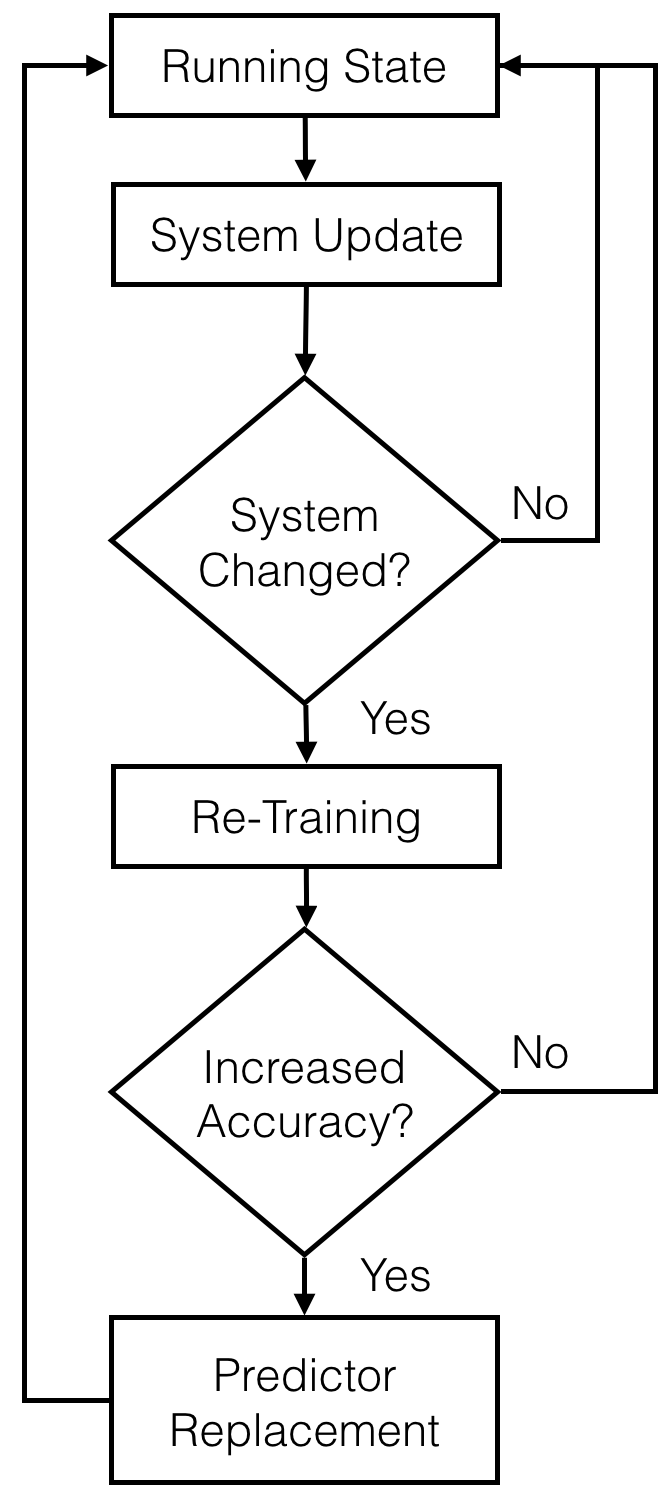
\includegraphics[width=#1]{ExecutionPhase}
    \caption[\ac{AFP} Execution Phase~\cite{irrera2015}]{The flow of the major
    steps involved in the \ac{AFP} framework execution
    phase~\cite{irrera2015}.}
    \label{fig:ExecutionPhase}
  \end{center}
\end{figure}
}


\newcommand{\figExecutionPhaseHoriz}[1]{\begin{figure}
  \begin{center}
    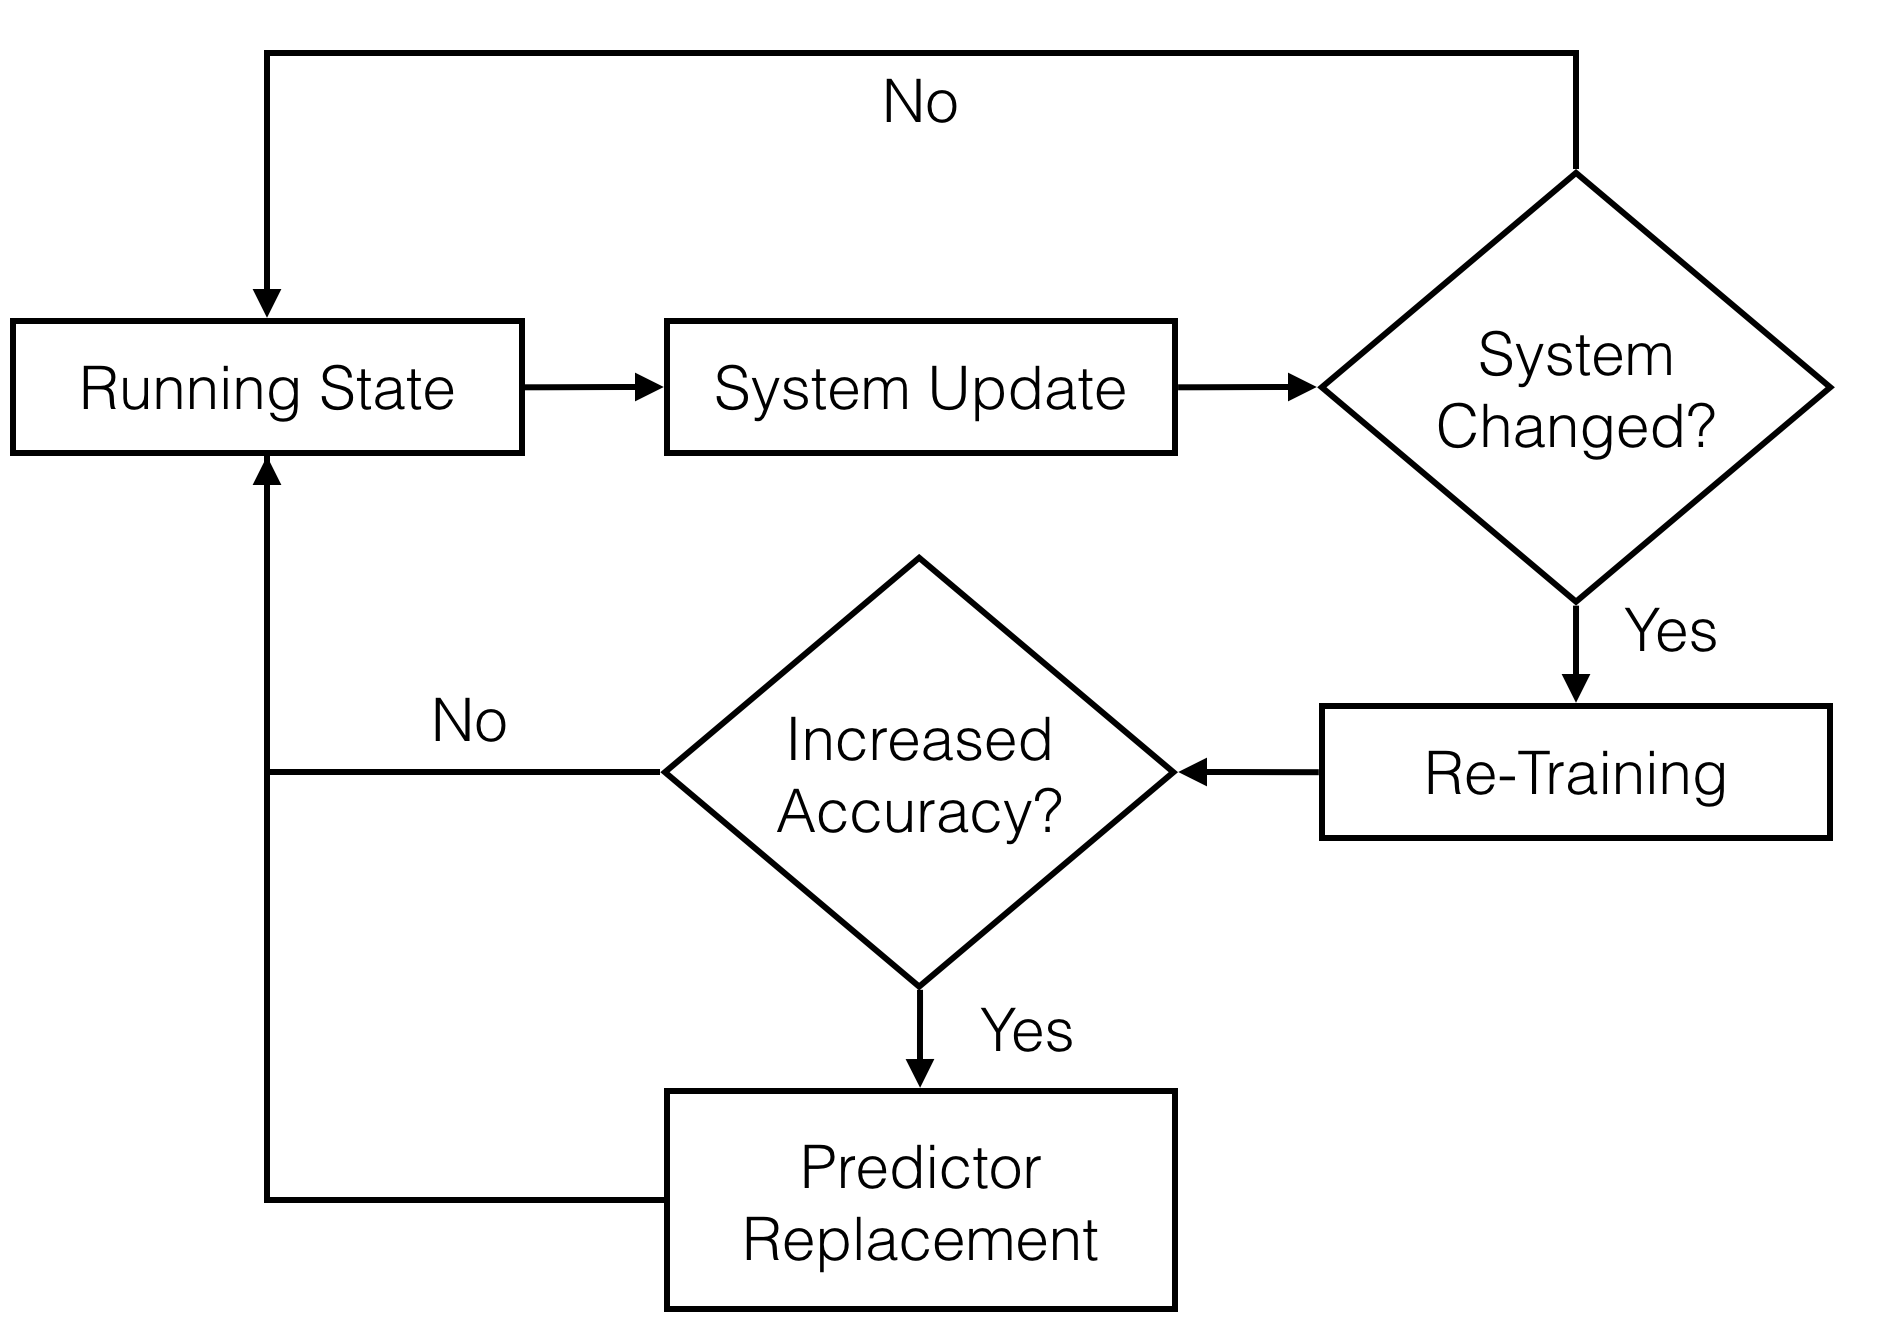
\includegraphics[width=#1]{ExecutionPhaseHoriz}
    \caption[\ac{AFP} Execution Phase~\cite{irrera2015}]{The flow of the major
    steps involved in the \ac{AFP} framework execution
    phase~\cite{irrera2015}.}
    \label{fig:ExecutionPhaseHoriz}
  \end{center}
\end{figure}
}

\newcommand{\figAuthDCPPS}[1]{\begin{figure}
 \begin{center}
  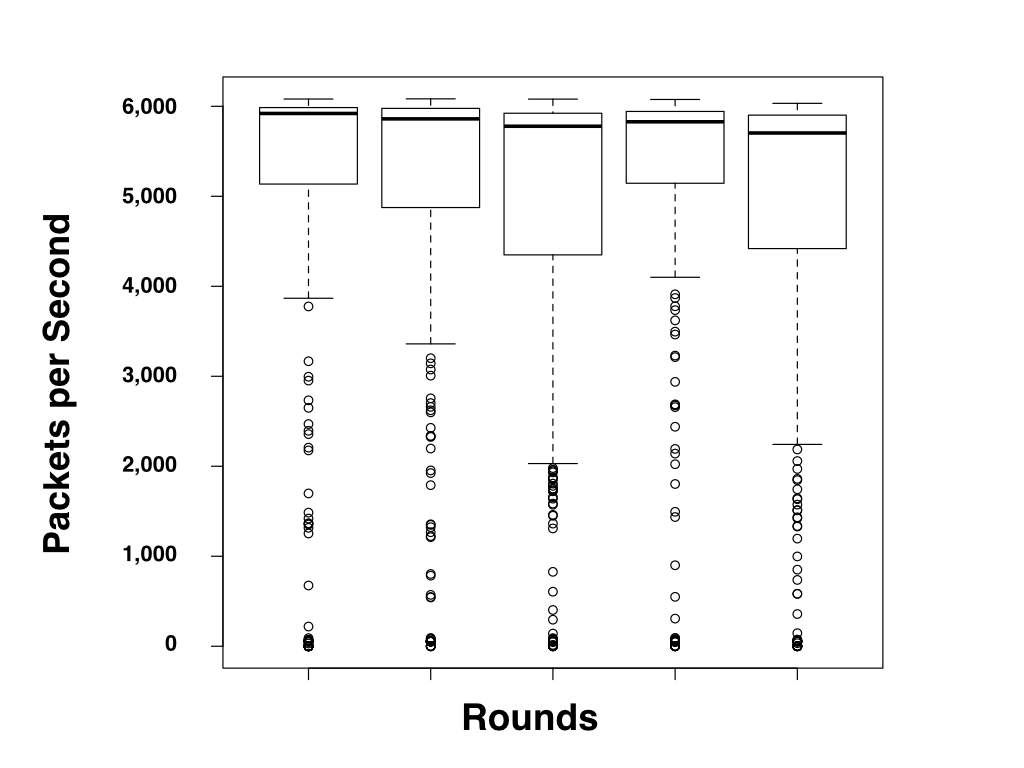
\includegraphics[width=#1]{DPLG/authDCPPS}
  \caption[Domain Controller Packets per Second]{How many packets per second
  were sent or received by the domain controller across all five rounds of the
  first test.  In each test, we captured approximately 1.8 million packets.}
  \label{fig:authDCPPS}
 \end{center}
\end{figure}
}

\newcommand{\figAuthClientPPS}[1]{\begin{figure}
 \begin{center}
  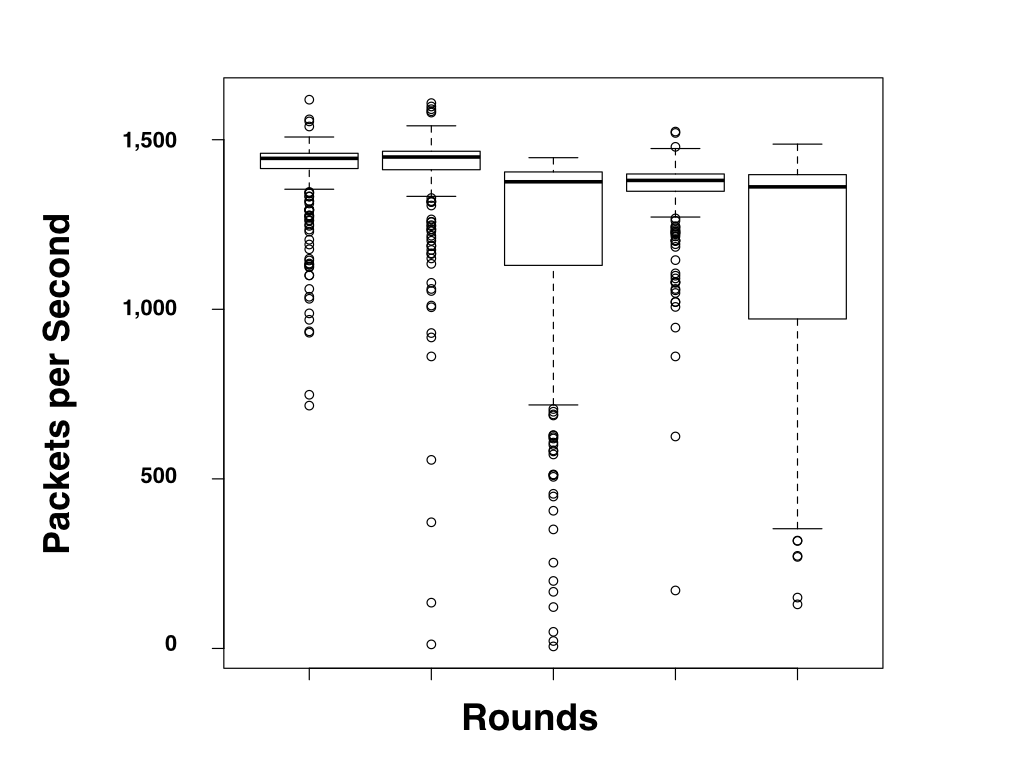
\includegraphics[width=#1]{DPLG/authClientPPS}
  \caption[Client Packets per Second]{How many packets per second were sent or
  received by one of the clients across all five rounds of the first test.}
  \label{fig:authClientPPS}
 \end{center}
\end{figure}
}

\newcommand{\figAuthDCMetrics}[1]{\begin{figure}
 \begin{center}
  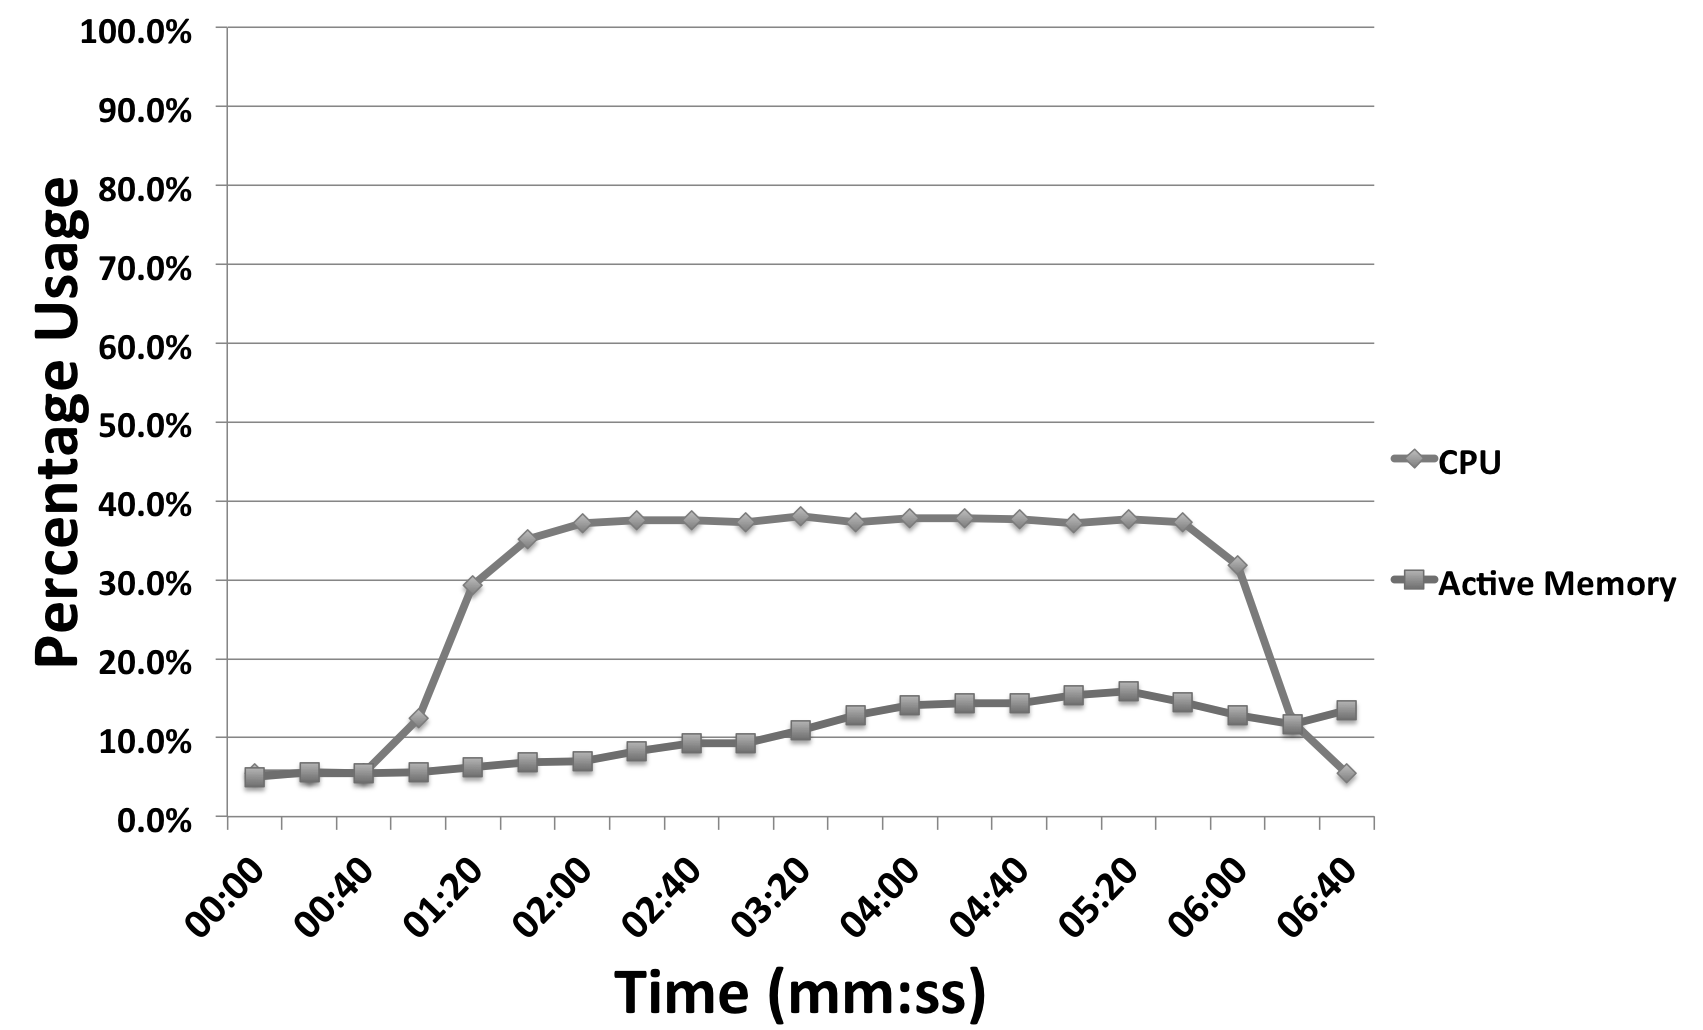
\includegraphics[width=#1]{DPLG/authDCMetrics}
  \caption[Test 1:  Domain Controller Performance]{Domain controller CPU and
  memory utilization during the first test.}
  \label{fig:authDCMetrics}
 \end{center}
\end{figure}
}

\newcommand{\figOFPTaxonomy}[1]{\begin{figure}
 \begin{center}
  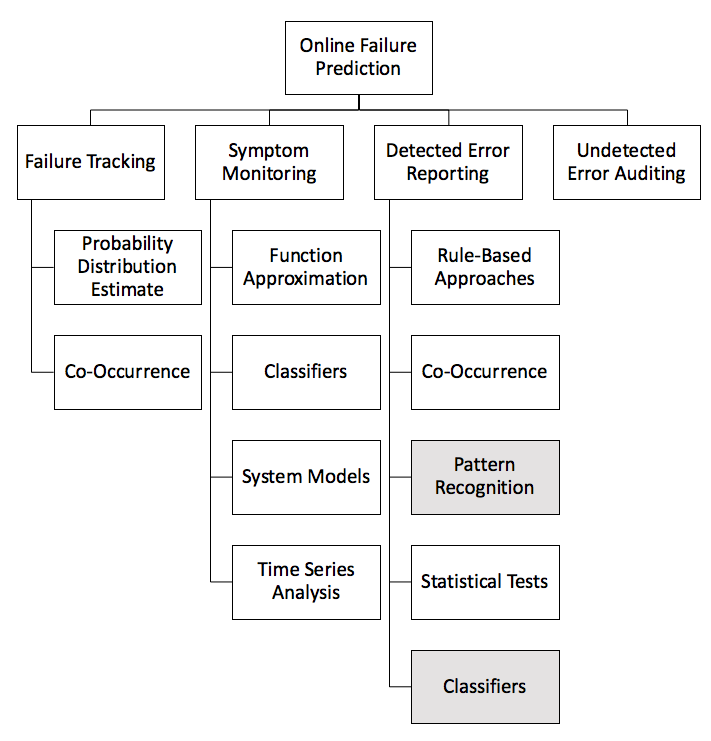
\includegraphics[width=#1]{OFPTaxonomy}
  \caption[Taxonomy of \ac{OFP} Approaches]{Taxonomy of approaches to online
  failure prediction~\cite{salfnerSurvey}.  The two categories into which this
  research falls are highlighted.}
  \label{fig:OFPTaxonomy}
 \end{center}
\end{figure}
}

\newcommand{\figMemLeakROC}[1]{\begin{figure}
 \begin{center}
  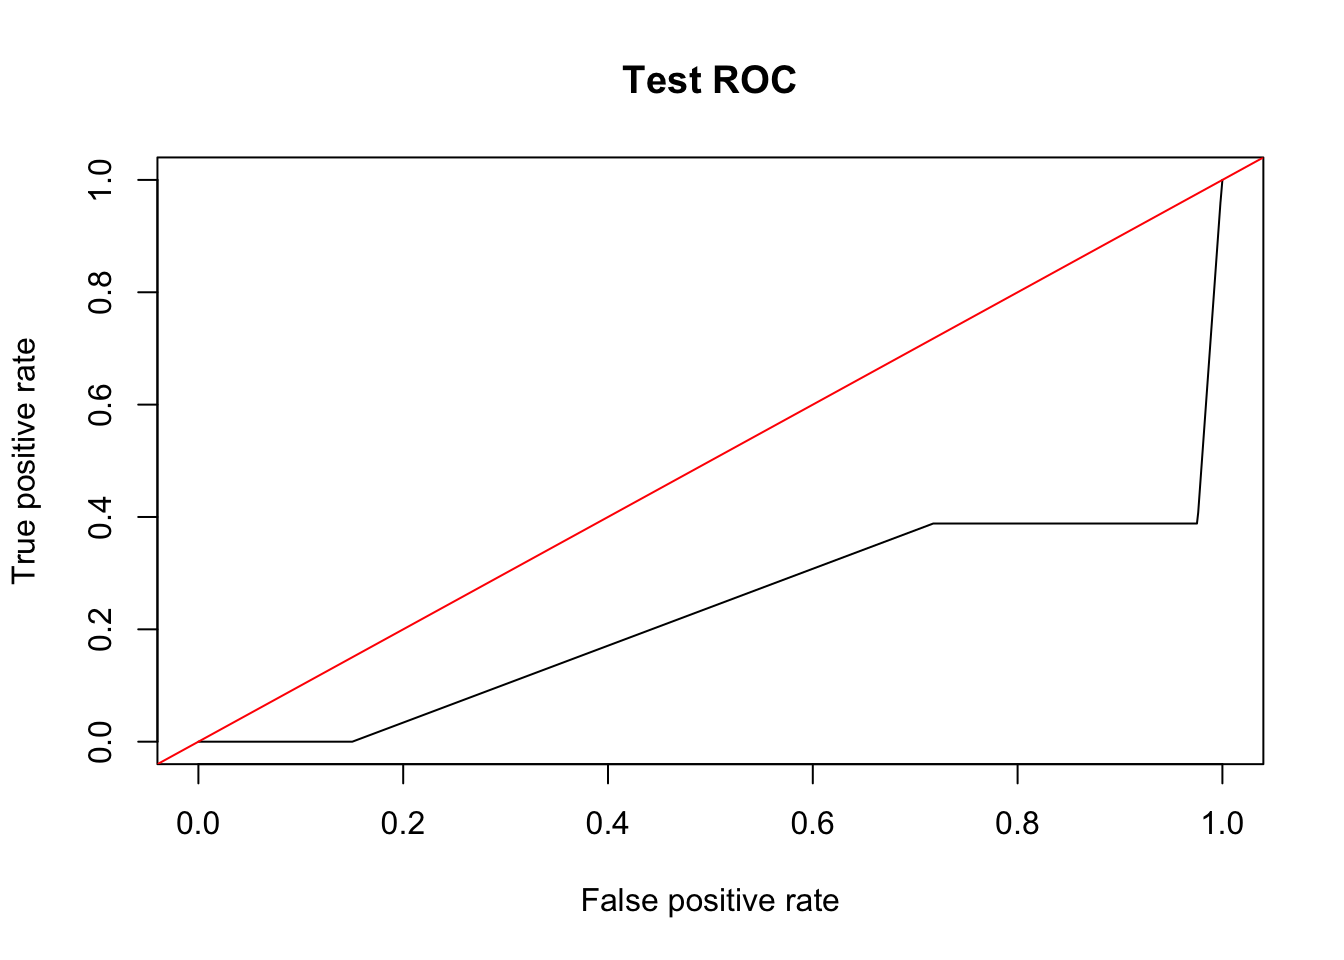
\includegraphics[width=#1]{MemLeakROC}
  \caption[\ac{SVM} Memory Leak \ac{ROC} Curve]{\ac{SVM} memory leak test data
  \ac{ROC} curve.}
  \label{fig:memLeakROC}
 \end{center}
\end{figure}
}

\newcommand{\figMemLeakCompare}[1]{\begin{figure}
 \begin{center}
  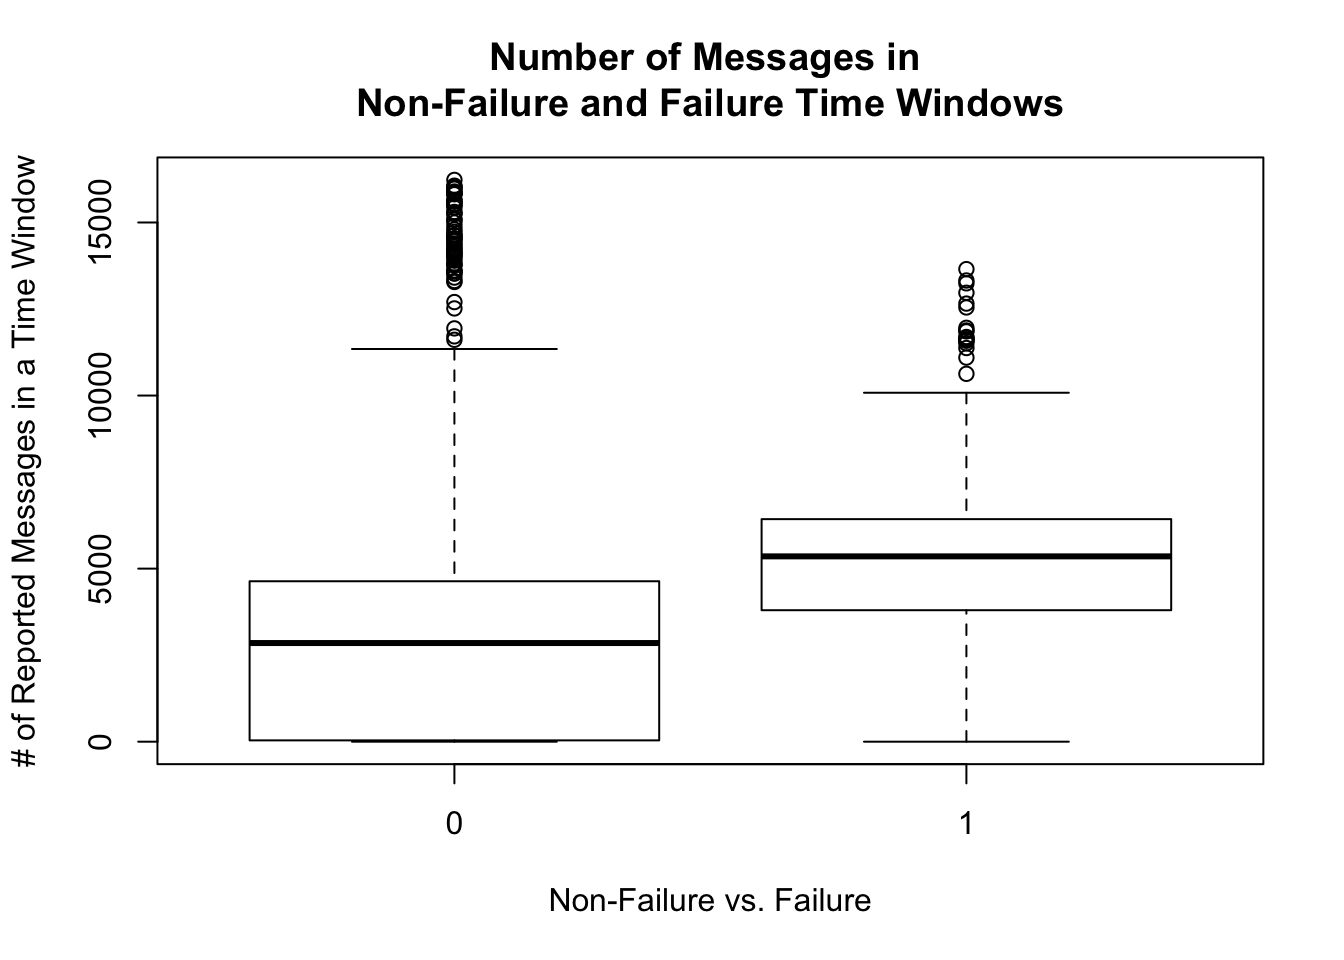
\includegraphics[width=#1]{MemLeakCompare}
  \caption[\ac{SVM} Memory Leak Performance Comparison]{Number of observations
  in a given thirty second time window where `1' represents a window during
  which failure occurred and `0' represents a window during which no failure
  occurred.}
  \label{fig:memLeakCompare}
 \end{center}
\end{figure}
}

%%%%   SMV   %%%%
% Pre-Update
\newcommand{\figMemLeakPreUpdateSVMPerf}{\begin{figure*}
  \centering
  \subfigure[Precision/Recall Curve.]{
    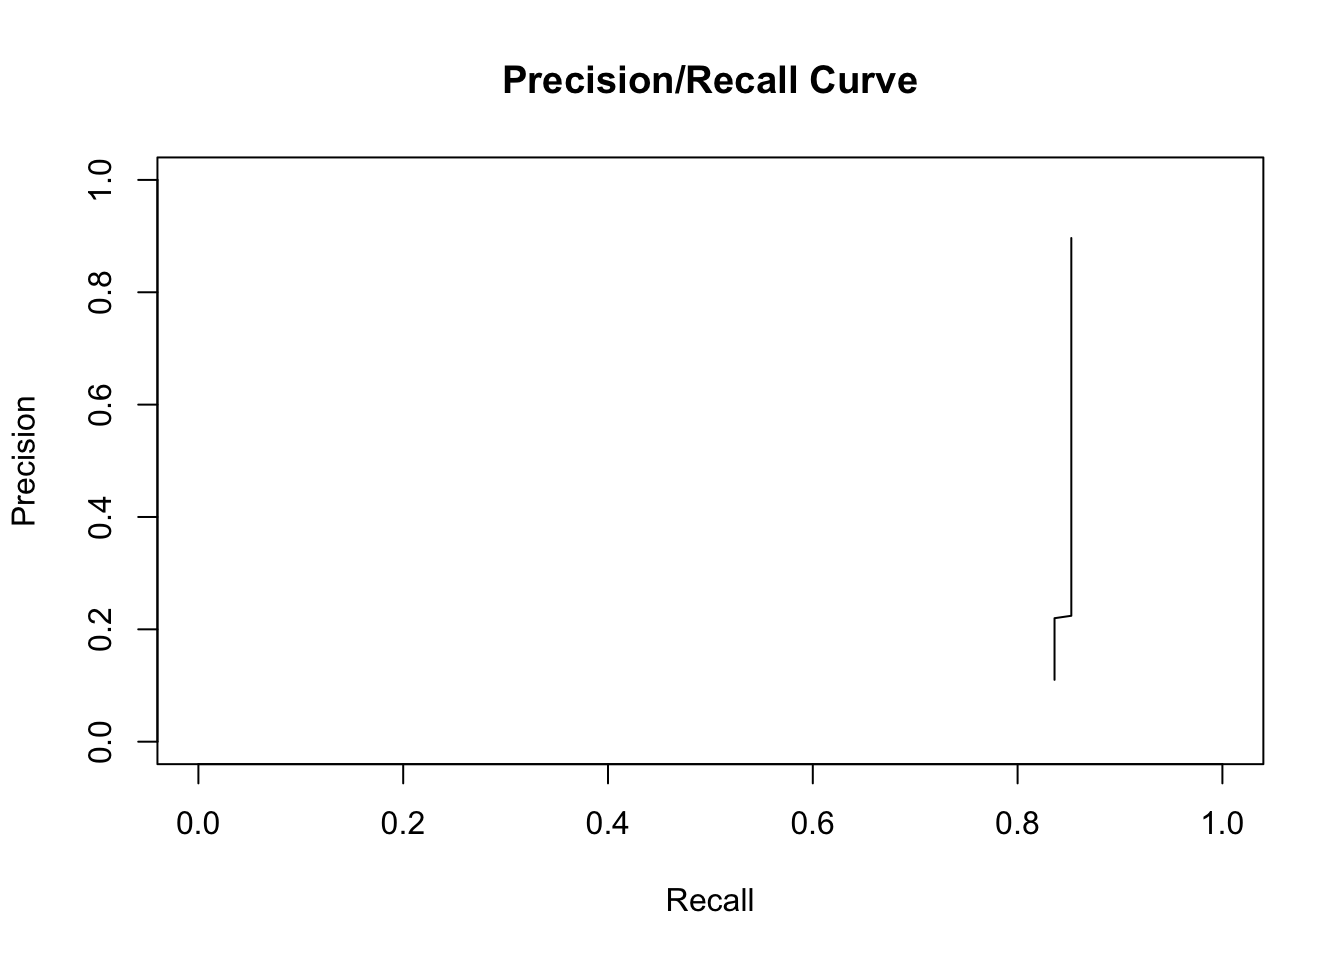
\includegraphics[width=0.45\textwidth]{results/pre-update/memleak/svm-prc}
  }
  \subfigure[\ac{ROC} Curve (\ac{AUC} = 0.8664).]{
    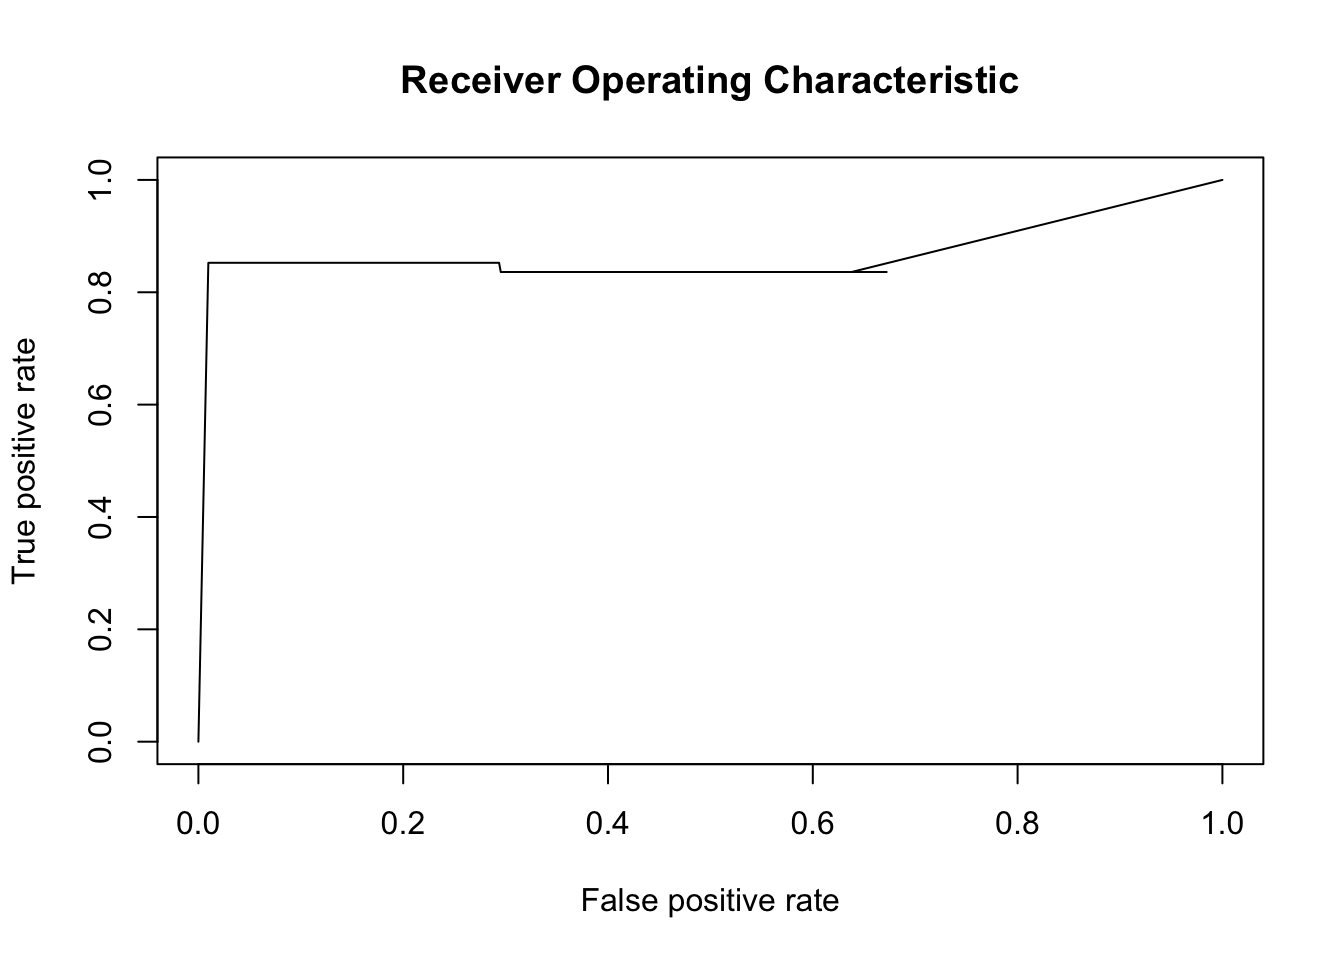
\includegraphics[width=0.45\textwidth]{results/pre-update/memleak/svm-roc}
  }
  \caption[Pre-Update, Memory Leak \ac{SVM} Performance]{Test data performance
  of the \ac{SVM} prediction method on failure data obtained by consuming all
  available memory until target application fails.}
  \label{fig:memLeakPreUpdateSVMPerf}
\end{figure*}
}

% Post-Update (old model)

% Post-Update New Model

%%%%   BOOSTING   %%%%
% Pre-Update
\newcommand{\figMemLeakPreUpdateBoostingPerf}{\begin{figure*}
  \centering
  \subfigure[Precision/Recall Curve.]{
    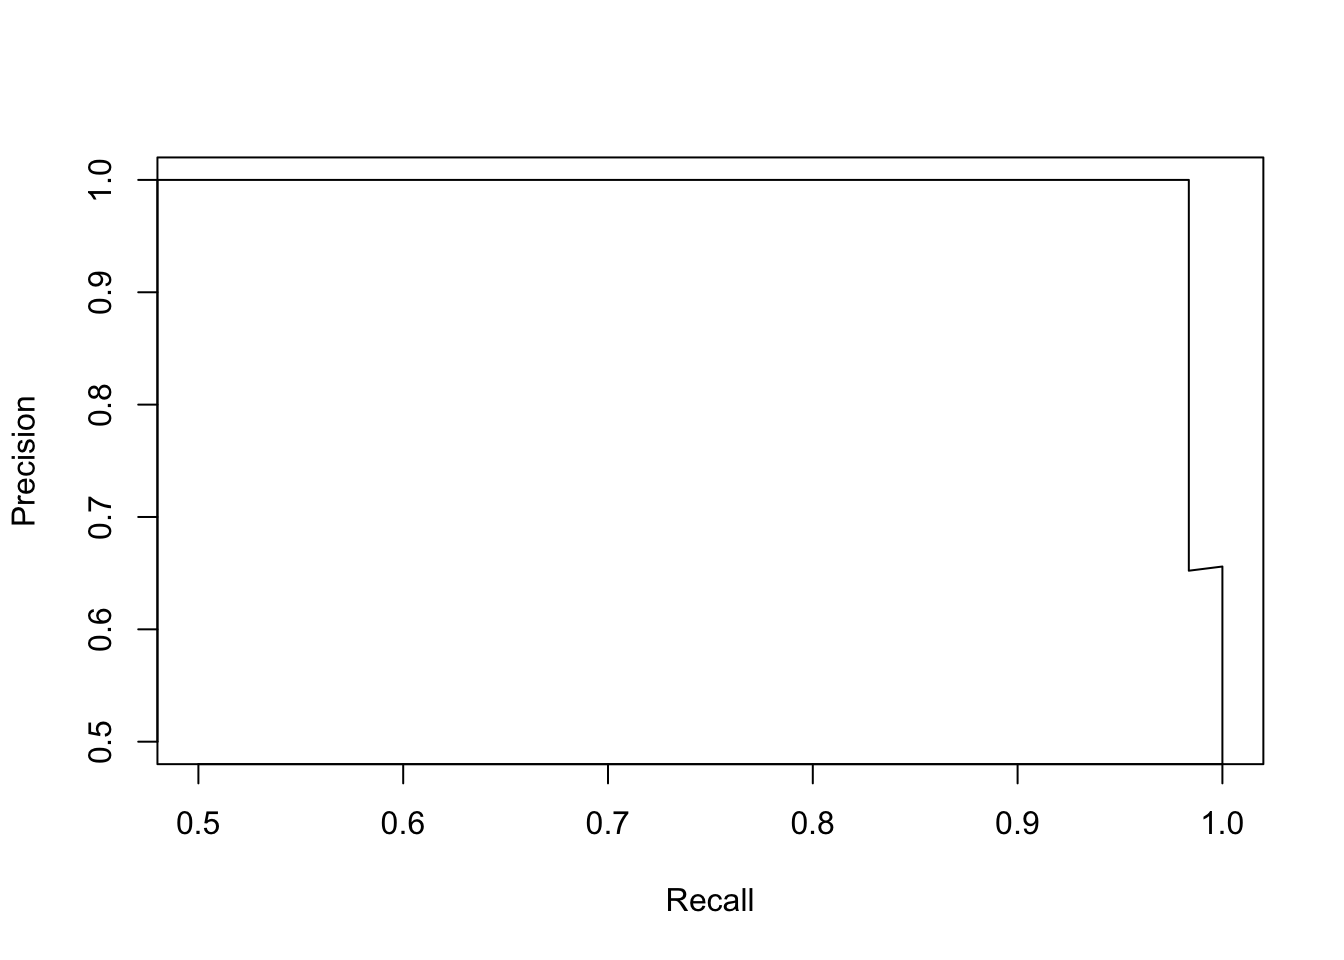
\includegraphics[width=0.45\textwidth]{results/pre-update/memleak/boosting-prc}
  }
  \subfigure[\ac{ROC} Curve (\ac{AUC} = 0.9984).]{
    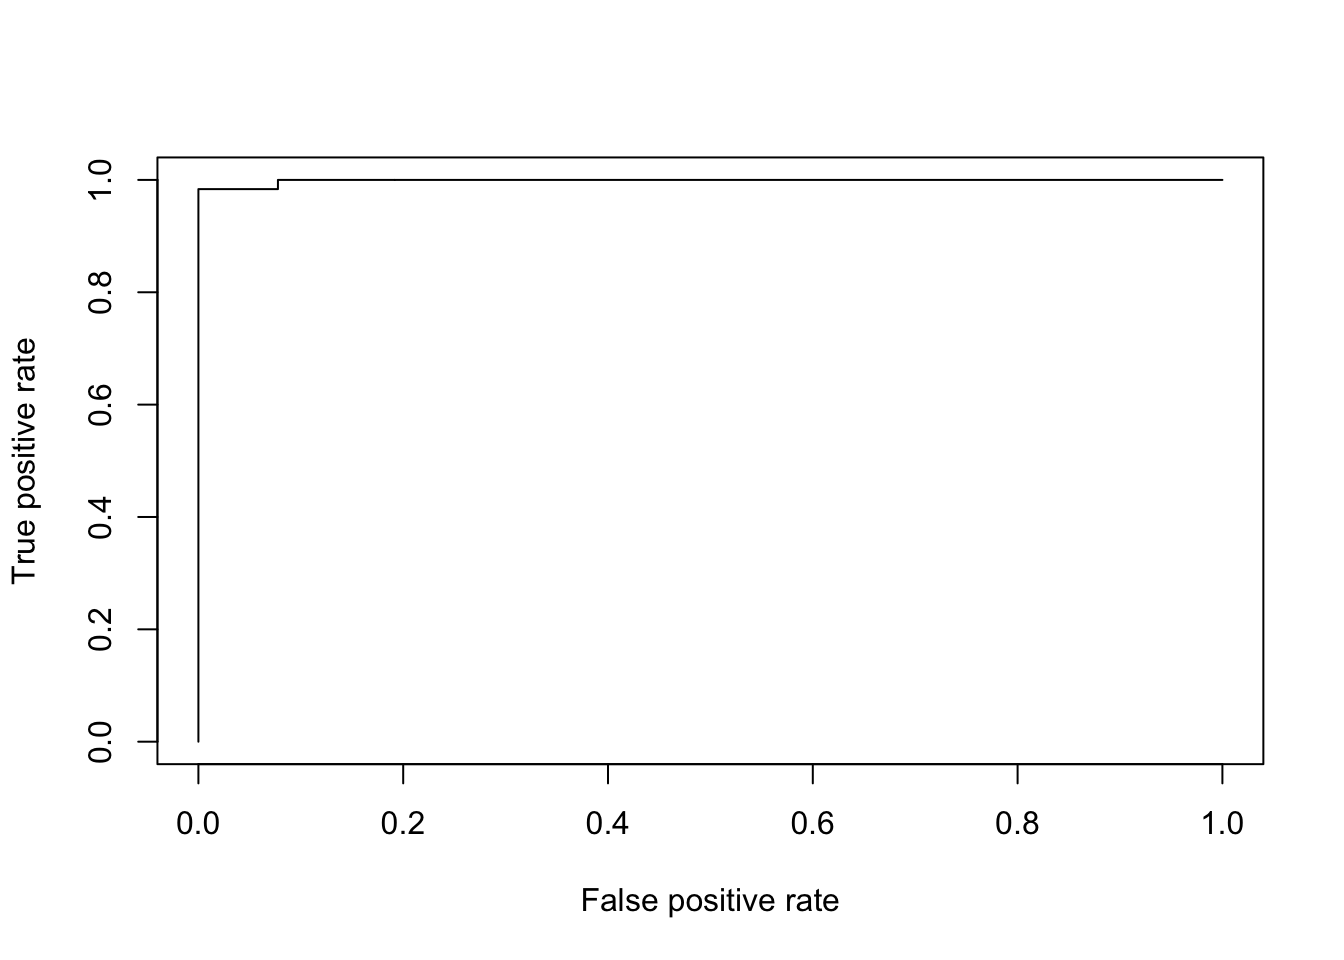
\includegraphics[width=0.45\textwidth]{results/pre-update/memleak/boosting-roc}
  }
  \caption[Pre-Update, Memory Leak Boosting Performance]{Test data performance
  of the boosting prediction method on failure data obtained by consuming all
  available memory until target application fails.}
  \label{fig:memLeakPreUpdateBoostingPerf}
\end{figure*}
}

% Post-Update (old model)
\newcommand{\figMemLeakPostUpdateSameBoostedModel}{\begin{figure*}
  \centering
  \subfigure[Precision/Recall Curve.]{
    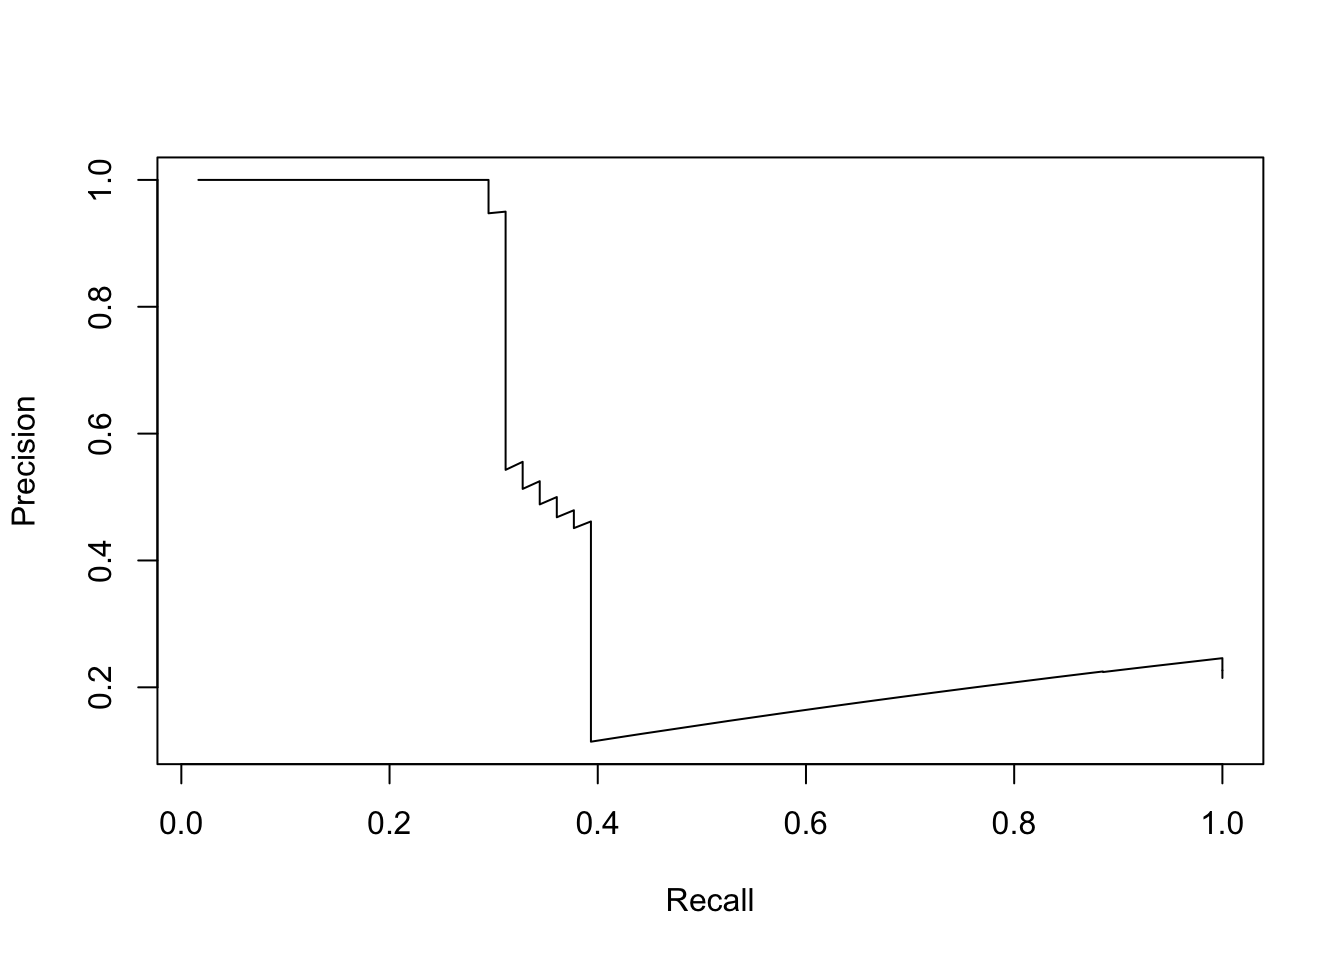
\includegraphics[width=0.45\textwidth]{results/post-update/memleak/boost-samemodel-prc}
  }
  \subfigure[\ac{ROC} Curve (\ac{AUC} = 0.4854).]{
    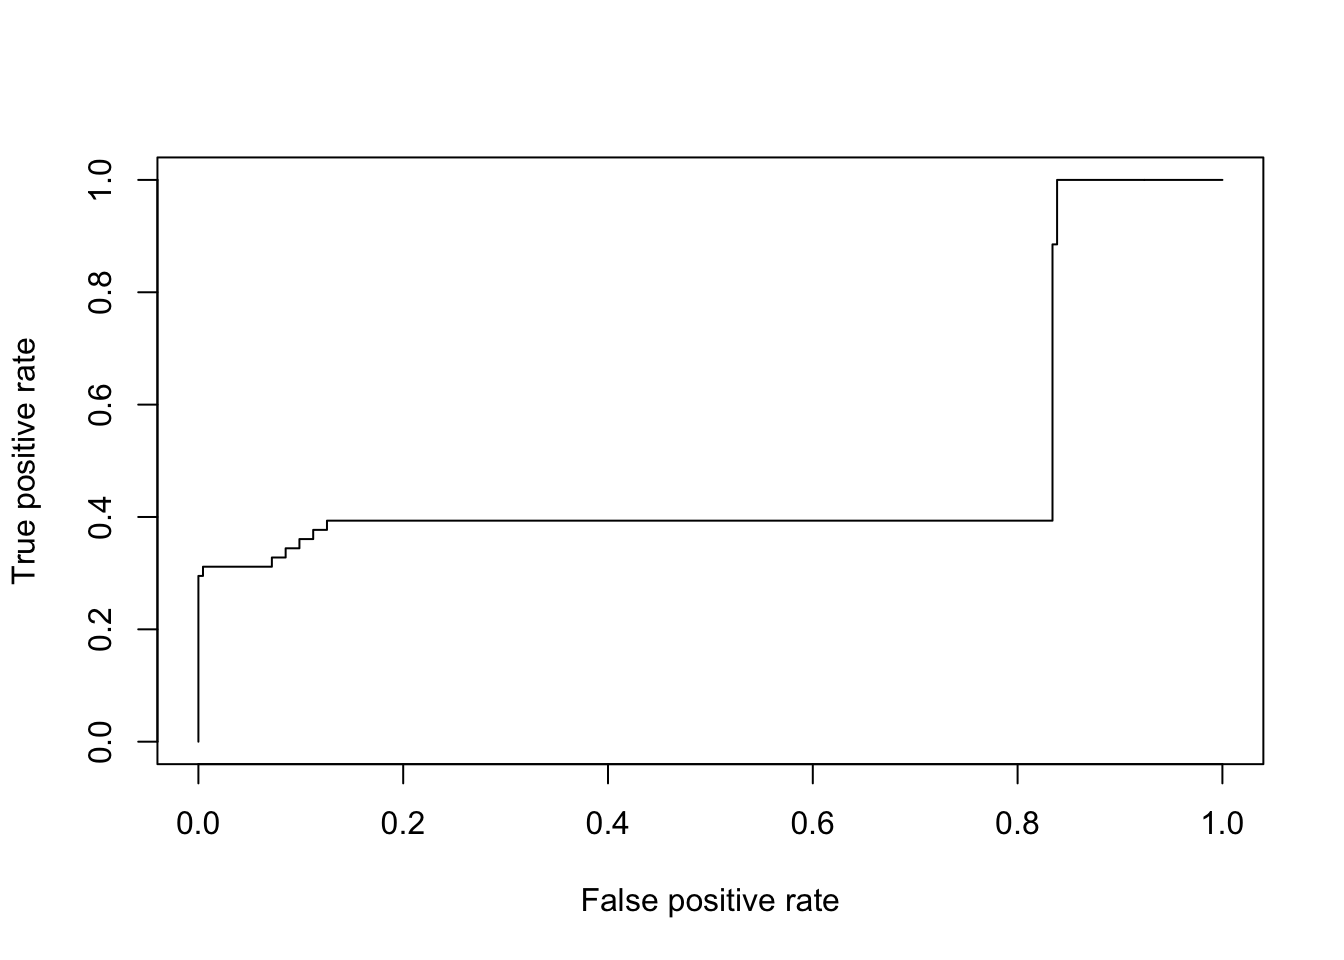
\includegraphics[width=0.45\textwidth]{results/post-update/memleak/boost-samemodel-roc}
  }
  \caption[Post-Update, Memory Leak Using Old Model Performance]{Performance of
  the boosting prediction method trained on failure data created before the
  software update obtained by consuming all available memory until target
  application fails.}
  \label{fig:memLeakPostUpdateSameBoostedModel}
\end{figure*}
}

% Post-Update New Model
\newcommand{\figMemLeakPostUpdateBoostingPerf}{\begin{figure*}
  \centering
  \subfigure[Precision/Recall Curve.]{
    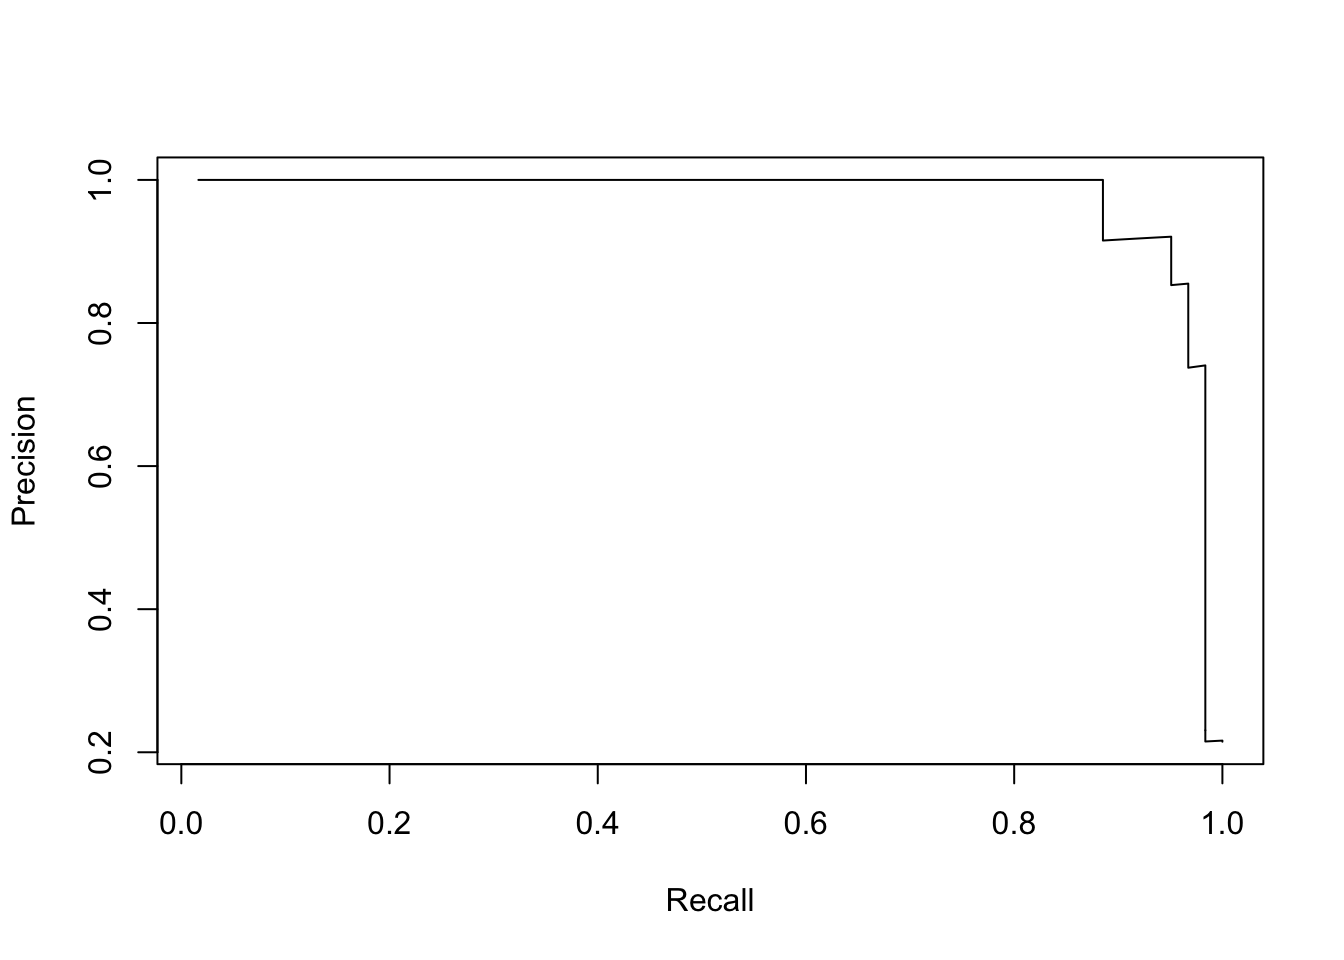
\includegraphics[width=0.45\textwidth]{results/post-update/memleak/boost-prc}
  }
  \subfigure[\ac{ROC} Curve (\ac{AUC} = 0.9801).]{
    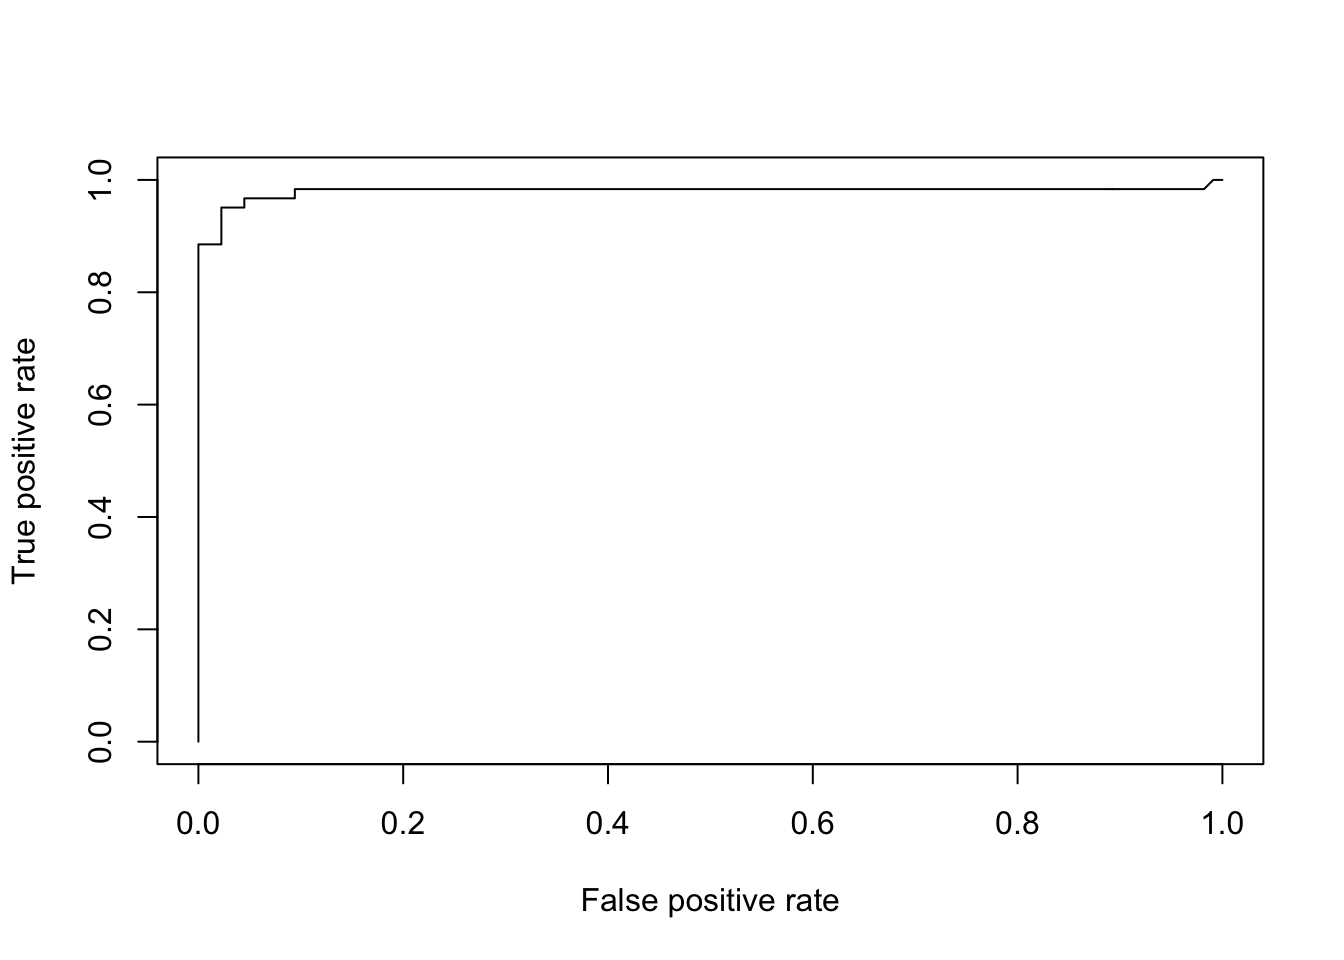
\includegraphics[width=0.45\textwidth]{results/post-update/memleak/boost-roc}
  }
  \caption[Post-Update, Memory Leak Using New Model Performance]{Performance of
  the boosting prediction method trained on failure data created after the
  software update obtained by consuming all available memory until target
  application fails.}
  \label{fig:memLeakPostUpdateBoostingPerf}
\end{figure*}
}

\newcommand{\figDPLGConceptDiagram}[1]{\begin{figure}
  \centering 
  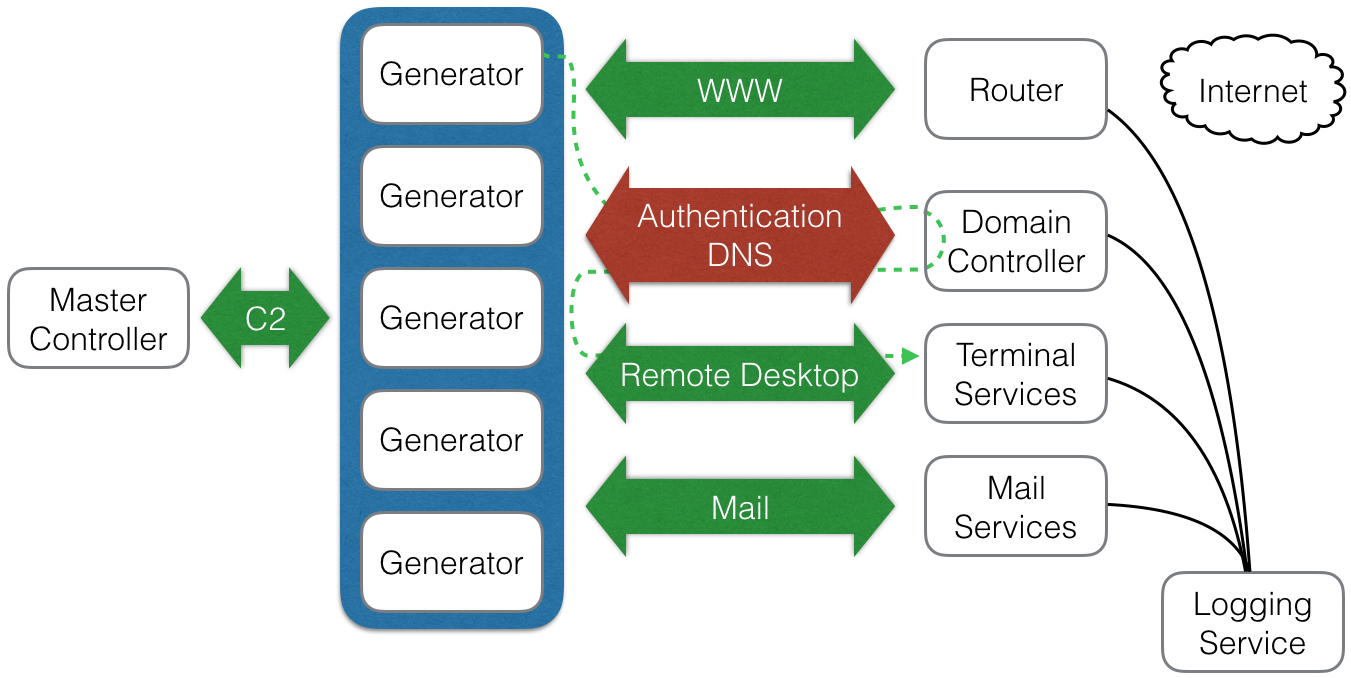
\includegraphics[width=#1]{DPLG/dplgConceptDiagram}
  \caption[Concept Diagram]{How each type of traffic that is generated is
  routed.  Log events are offloaded to logging service for further analysis.}
  \label{fig:conceptDiagram} 
  \end{figure}
}

\newcommand{\figDPLGAllModsClientMetrics}[1]{\begin{figure}
  \centering
  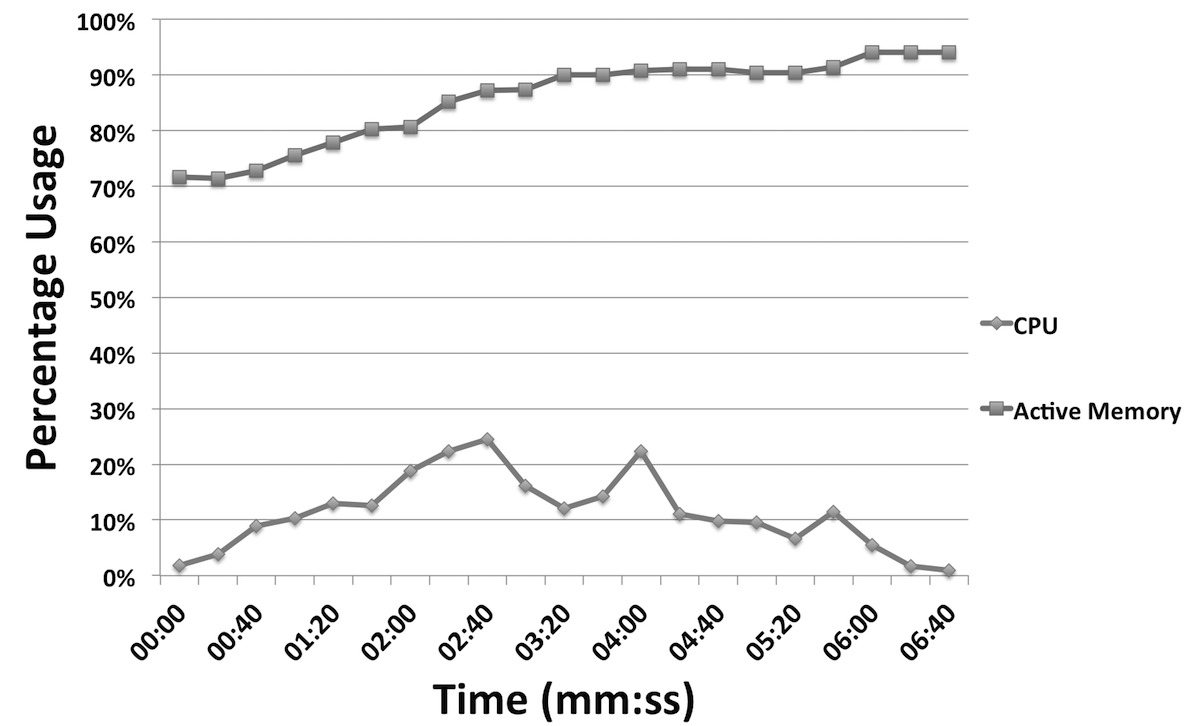
\includegraphics[width=#1]{DPLG/allModsClientMetrics}
  \caption[Test 2:  Client Metrics]{Client CPU and memory utilization during
  the second test.} \label{fig:allModsClientMetrics}
  \end{figure}
}


\newcommand{\tabFaults}{
\begin{table}[htbp]
  \centering
  \caption{Table of Faults Injected~\cite{gswfit}.}\label{tab:faults}
\begin{tabular}{ | c | l | c | } 
\hline
	\textbf{Type}  & \textbf{Description}  & \textbf{ODC Classes}  \\ \hline \hline
	MIFS  & Missing "If (cond) \{ statement(s) \}"  & Algorithm  \\ \hline
	MFC  & Missing function call  & Algorithm  \\ \hline
	MLAC  & Missing "AND EXPR" in expression used as branch & Checking  \\ \hline
	MLPC  & Missing small and localized part of the algorithm  & Algorithm  \\ \hline
	WVAV  & Wrong value assigned to a value  & Assignment  \\ \hline
	MVI  & Missing variable initialization  & Assignment  \\ \hline
	MVAV  & Missing variable assignment using a value  & Assignment  \\ \hline
	WPFV  & Wrong variable used in parameter of function call  & Interface  \\ \hline
\end{tabular}
\end{table}
}

\newcommand{\tabTranslationThirtyTwo}{
\begin{table}[htbp]
  \centering
  \caption{Funtion Entry/Exit Patterns
  (IA32)~\cite{gswfit}.}\label{tab:translationThirtyTwo}
\begin{tabular}{ | l | l | l | l | }
\hline
	\multicolumn{2}{|c|}{\textbf{Module Entry Point}}& 
  \multicolumn{2}{c|}{\textbf{Module Exit Point}} \\ \hline

	\textbf{Instruction Sequence} & \textbf{Explanation} &
  \textbf{Instruction Sequence} & \textbf{Explanation} \\ \hline \hline

	push ebp & stack frame & move esp,ebp & stack frame \\ \hline
	mov ebp, esp & setup & pop ebp & cleanup \\ \hline
	sub esp, \emph{immed} &  & ret &  \\ \hline
\end{tabular}
\end{table}
}

\newcommand{\tabTranslationSixtyFour}{
\begin{table}[htbp]
  \centering
  \caption{Funtion Entry/Exit Patterns
  (x86-64)~\cite{gswfit}.}\label{tab:translationSixtyFour}
\begin{tabular}{ | l | l | l | l | }
\hline
	\multicolumn{2}{|c|}{\textbf{Module Entry Point}}& 
  \multicolumn{2}{c|}{\textbf{Module Exit Point}} \\ \hline

	\textbf{Instruction Sequence} & \textbf{Explanation} & 
  \textbf{Instruction Sequence} & \textbf{Explanation} \\ \hline \hline

	push rbp & stack frame & add rsp, \emph{immed} & stack frame \\ \hline
	sub rsp, \emph{immed} &  & pop rbp & cleanup \\ \hline
	mov rbp, rdx & setup & ret &  \\ \hline
\end{tabular}
\end{table}
}

\newcommand{\tabHypervisorOne}{
\begin{table}[htbp]
  \centering
  \caption{Hypervisor 1 Configuration (Sandbox/Target).} \label{tab:hyp1}
  \begin{tabular}{ | c | l | l | c | l |}
    \hline
    Qty. & Role   & Operating System    & CPU / Mem. \\ \hline\hline
    1    & DC     & Win. Server 2008 R2 & 2 / 2 GB   \\ \hline
    5    & Client & Win. 7              & 1 / 512 MB \\ 
    \hline
  \end{tabular}
\end{table}
}


\newcommand{\tabHypervisorTwo}{
\begin{table}[htbp]
  \centering
  \caption{Hypervisor 2 Configuration (Controller).} \label{tab:hyp2}
  \begin{tabular}{ | c | l | l | c | l |}
    \hline
    Qty. & Role & Operating System    & CPU / Mem. \\ \hline\hline
    1    & RDP  & Win. Server 2008 R2 & 1 / 4 GB   \\ \hline
    1    & Log  & Ubuntu 14.04 LTS    & 1 / 1 GB   \\ 
    \hline
  \end{tabular}
\end{table}
}

\newcommand{\tabMessage}{
\begin{table}[!ht] \centering
  \caption{Typical authentication message sent as keys that correspond to the
  values as designated in the \emph{Snare} protocol for MSWinEventLog used by
  the SolarWinds syslog agent.} \label{tab:message}
  \begin{tabular}{ | l | l | }
    \hline
      Key                 & Value                               \\ \hline\hline
      HostName            & dc.afnet.com                        \\ \hline
      Criticality         & 5                                   \\ \hline
      EventLogSource      & Security                            \\ \hline
      Counter             & 3                                   \\ \hline
      SubmitTime          & Sun May 08 14:31:50 2016            \\ \hline
      EventID             & 4672                                \\ \hline
      SourceName          & Microsoft-Windows-Security-Auditing \\ \hline
      UserName            & N/A                                 \\ \hline
      SIDType             & Audit Success                       \\ \hline
      EventLogType        & dc.afnet.com                        \\ \hline
      ComputerName        & 12548                               \\ \hline
      CategoryString      & Special privileges assigned to\dots \\ \hline
      ExtendedDataString  & Security ID:  S-1-5-21-2379403\dots \\ 
    \hline
  \end{tabular}
\end{table}
}

\newcommand{\tabSlidingWindow}{
\begin{table}[!ht] \centering
  \caption{Sample time window after message translation.} \label{tab:window}
  \begin{tabular}{ | l | l | }
    \hline
      Key                         & Value \\ \hline\hline
      FailureWindow               & 0     \\ \hline
      NumObservations             & 2     \\ \hline
      Criticality: 6              & 2     \\ \hline
      Criticality: 2              & 0     \\ \hline
      Criticality: 4              & 0     \\ \hline
      EventLogSource: Application & 1     \\ \hline
      EventLogSource: System      & 1     \\ 
    \hline
  \end{tabular}
\end{table}
}

\newcommand{\tabMemLeakPreUpdateSVMStats}{
\begin{table}[!t] \centering
  \caption[Pre-Update, Memory Leak, SVM Statistics]{Classification statistics
  on test data created before software updates.}
  \label{tab:memLeakPreUpdateSVMStats}
  \begin{tabular}{ | l | l | }
    \hline
      Statistic           & Value  \\ \hline\hline
      True Positive Rate  & 0.8525 \\ \hline
      False Positive Rate & 0.0098 \\ \hline
      Accuracy            & 0.9777 \\ \hline
      Precision           & 0.8966 \\ \hline
      Recall              & 0.8525 \\ \hline
      F-Measure           & 0.8739 \\
    \hline
  \end{tabular}
\end{table}
}
%%%%%%%%%%%%%%%%%%%%%%%%%%%%%%%%%%%%%%%%%%%%%%%%%%%%%%%%%%%%%%%%%%%%%%%%%%%%%%%
%%%%   SVM   %%%%
% Pre-Update
\newcommand{\tabMemLeakPreUpdateSVMConfusionMatrix}{
  \begin{table}[!ht]
    \centering
    \caption[Pre-Update, Memory Leak, SVM Confusion Matrix]{Confusion matrix on
    test data created before software updates on threshold with highest
    F-Measure (0.8739) using SVM.}
    \label{tab:memLeakPreUpdateSVMConfusionMatrix}
    \begin{tabular}{llll}
                                                               &                                       & \multicolumn{2}{c}{\textbf{Actual}}                                        \\ \cline{3-4} 
                                                               & \multicolumn{1}{l|}{}                 & \multicolumn{1}{l|}{\textbf{Fail}} & \multicolumn{1}{l|}{\textbf{No-Fail}} \\ \cline{2-4} 
      \multicolumn{1}{c|}{\multirow{2}{*}{\textbf{Predicted}}} & \multicolumn{1}{l|}{\textbf{Fail}}    & \multicolumn{1}{l|}{52}            & \multicolumn{1}{l|}{6}                \\ \cline{2-4} 
      \multicolumn{1}{c|}{}                                    & \multicolumn{1}{l|}{\textbf{No-Fail}} & \multicolumn{1}{l|}{9}             & \multicolumn{1}{l|}{607}              \\ \cline{2-4} 
    \end{tabular}
  \end{table}
}

% Post-Update (old model)

% Post-Update New Model

%%%%   BOOSTING   %%%%
% Pre-Update
\newcommand{\tabMemLeakPreUpdateBoostingConfusionMatrix}{
  \begin{table}[!ht]
    \centering
    \caption[Pre-Update, Memory Leak, Boosting Confusion Matrix]{Confusion
    matrix on test data created before software updates on threshold with
    highest F-Measure (0.9917) using boosting.}
    \label{tab:memLeakPreUpdateBoostingConfusionMatrix}
    \begin{tabular}{llll}
                                                               &                                       & \multicolumn{2}{c}{\textbf{Actual}}                                        \\ \cline{3-4} 
                                                               & \multicolumn{1}{l|}{}                 & \multicolumn{1}{l|}{\textbf{Fail}} & \multicolumn{1}{l|}{\textbf{No-Fail}} \\ \cline{2-4} 
      \multicolumn{1}{c|}{\multirow{2}{*}{\textbf{Predicted}}} & \multicolumn{1}{l|}{\textbf{Fail}}    & \multicolumn{1}{l|}{60}            & \multicolumn{1}{l|}{0}                \\ \cline{2-4} 
      \multicolumn{1}{c|}{}                                    & \multicolumn{1}{l|}{\textbf{No-Fail}} & \multicolumn{1}{l|}{1}             & \multicolumn{1}{l|}{412}              \\ \cline{2-4} 
    \end{tabular}
  \end{table}
}

% Post-Update (old model)
\newcommand{\tabMemLeakPostUpdateBoostingSameModelConfusionMatrix}{
  \begin{table}[!ht]
    \centering
    \caption[Post-Update, Memory Leak, Same Model, Confusion
    Matrix]{Post-update failure data confusion matrix on threshold with highest
    F-Measure (0.4691) using model trained on failure data generated before
    software update.}
    \label{tab:memLeakPostUpdateBoostingSameModelConfusionMatrix}
    \begin{tabular}{llll}
                                                               &                                       & \multicolumn{2}{c}{\textbf{Actual}}                                        \\ \cline{3-4} 
                                                               & \multicolumn{1}{l|}{}                 & \multicolumn{1}{l|}{\textbf{Fail}} & \multicolumn{1}{l|}{\textbf{No-Fail}} \\ \cline{2-4} 
      \multicolumn{1}{c|}{\multirow{2}{*}{\textbf{Predicted}}} & \multicolumn{1}{l|}{\textbf{Fail}}    & \multicolumn{1}{l|}{19}            & \multicolumn{1}{l|}{1}                \\ \cline{2-4} 
      \multicolumn{1}{c|}{}                                    & \multicolumn{1}{l|}{\textbf{No-Fail}} & \multicolumn{1}{l|}{42}            & \multicolumn{1}{l|}{222}              \\ \cline{2-4} 
    \end{tabular}
  \end{table}
}

% Post-Update New Model
\newcommand{\tabMemLeakPostUpdateBoostingConfusionMatrix}{
  \begin{table}[!ht]
    \centering
    \caption[Post-Update, Memory Leak, New Model, Confusion
    Matrix]{Post-update failure data confusion matrix on threshold with highest
    F-Measure (0.9355) using model trained on failure data generated after
    software update.}
    \label{tab:memLeakPostUpdateBoostingConfusionMatrix}
    \begin{tabular}{llll}
                                                               &                                       & \multicolumn{2}{c}{\textbf{Actual}}                                        \\ \cline{3-4} 
                                                               & \multicolumn{1}{l|}{}                 & \multicolumn{1}{l|}{\textbf{Fail}} & \multicolumn{1}{l|}{\textbf{No-Fail}} \\ \cline{2-4} 
      \multicolumn{1}{c|}{\multirow{2}{*}{\textbf{Predicted}}} & \multicolumn{1}{l|}{\textbf{Fail}}    & \multicolumn{1}{l|}{58}            & \multicolumn{1}{l|}{5}                \\ \cline{2-4} 
      \multicolumn{1}{c|}{}                                    & \multicolumn{1}{l|}{\textbf{No-Fail}} & \multicolumn{1}{l|}{3}             & \multicolumn{1}{l|}{218}              \\ \cline{2-4} 
    \end{tabular}
  \end{table}
}

%%%%%%%%%%%%%%%%%%%%%%%%%%%%%%%%%%%%%%%%%%%%%%%%%%%%%%%%%%%%%%%%%%%%%%%%%%%%%%%
\newcommand{\tabModelSelection}{
\begin{table*}[!t]
  \centering
  \caption{Cross-validation runs on training data for model selection and
  resulting classification accuracy.}
  \label{tab:model:selection}
  \begin{tabular}{cllllllllllll}
    \multicolumn{1}{l}{}                       & \multicolumn{12}{c}{{\ul \textbf{Amount of Training Data}}}                                                                                                                                                                                         \\ \cline{2-13} 
    \multicolumn{1}{l|}{{\ul \textbf{Window}}} & \multicolumn{4}{c}{One Failure}                                             & \multicolumn{4}{c}{Two Failures}                                                & \multicolumn{4}{c|}{Four Failures}                                              \\ \cline{2-13} 
    \multicolumn{1}{c|}{\multirow{2}{*}{30s}}  & \textbf{Linear:}  & 0.0557 & \textbf{Poly:}   & \multicolumn{1}{l|}{0.0523} & \textbf{Linear:}  & 0.0756 & \textbf{Poly:}   & \multicolumn{1}{l|}{0.0659} & \textbf{Linear:}  & 0.0733 & \textbf{Poly:}   & \multicolumn{1}{l|}{0.0547} \\
    \multicolumn{1}{c|}{}                      & \textbf{Sigmoid:} & 0.0626 & \textbf{Radial:} & \multicolumn{1}{l|}{0.0459} & \textbf{Sigmoid:} & 0.0591 & \textbf{Radial:} & \multicolumn{1}{l|}{0.0438} & \textbf{Sigmoid:} & 0.0794 & \textbf{Radial:} & \multicolumn{1}{l|}{0.0542} \\ \cline{2-13} 
    \multicolumn{1}{c|}{\multirow{2}{*}{60s}}  & \textbf{Linear:}  & 0.0628 & \textbf{Poly:}   & \multicolumn{1}{l|}{0.0662} & \textbf{Linear:}  & 0.0779 & \textbf{Poly:}   & \multicolumn{1}{l|}{0.064}  & \textbf{Linear:}  & 0.0791 & \textbf{Poly:}   & \multicolumn{1}{l|}{0.0779} \\
    \multicolumn{1}{c|}{}                      & \textbf{Sigmoid:} & 0.1084 & \textbf{Radial:} & \multicolumn{1}{l|}{0.0487} & \textbf{Sigmoid:} & 0.1328 & \textbf{Radial:} & \multicolumn{1}{l|}{0.071}  & \textbf{Sigmoid:} & 0.2159 & \textbf{Radial:} & \multicolumn{1}{l|}{0.0797} \\ \cline{2-13} 
    \multicolumn{1}{c|}{\multirow{2}{*}{90s}}  & \textbf{Linear:}  & 0.1272 & \textbf{Poly:}   & \multicolumn{1}{l|}{0.0897} & \textbf{Linear:}  & 0.1131 & \textbf{Poly:}   & \multicolumn{1}{l|}{0.0732} & \textbf{Linear:}  & 0.0826 & \textbf{Poly:}   & \multicolumn{1}{l|}{0.0543} \\
    \multicolumn{1}{c|}{}                      & \textbf{Sigmoid:} & 0.1792 & \textbf{Radial:} & \multicolumn{1}{l|}{0.0779} & \textbf{Sigmoid:} & 0.2684 & \textbf{Radial:} & \multicolumn{1}{l|}{0.0757} & \textbf{Sigmoid:} & 0.2404 & \textbf{Radial:} & \multicolumn{1}{l|}{0.0552} \\ \cline{2-13} 
    \multicolumn{1}{c|}{\multirow{2}{*}{120s}} & \textbf{Linear:}  & 0.132  & \textbf{Poly:}   & \multicolumn{1}{l|}{0.104}  & \textbf{Linear:}  & 0.1452 & \textbf{Poly:}   & \multicolumn{1}{l|}{0.0785} & \textbf{Linear:}  & 0.0998 & \textbf{Poly:}   & \multicolumn{1}{l|}{0.0705} \\
    \multicolumn{1}{c|}{}                      & \textbf{Sigmoid:} & 0.204  & \textbf{Radial:} & \multicolumn{1}{l|}{0.104}  & \textbf{Sigmoid:} & 0.2864 & \textbf{Radial:} & \multicolumn{1}{l|}{0.0585} & \textbf{Sigmoid:} & 0.3056 & \textbf{Radial:} & \multicolumn{1}{l|}{0.0792} \\ \cline{2-13} 
  \end{tabular}
\end{table*}
}

% define custom commands
\newcommand{\regmark}{\raisebox{5pt}{\tiny \circledR}\xspace}
\newcommand{\matlab}{\textsc{Matlab}\regmark}
\newcommand{\trademark}{\raisebox{5pt}{\tiny TM}\xspace}
\newcommand{\mca}{\texttt{Mathematica}\regmark}
\newcommand{\Latex}{\LaTeX\xspace}

% Create a new theorem style called a Corollary.
% If you don't have any, then just comment this out.
%\theoremstyle{plain} % Default
\newtheorem{cor}{Corollary}[chapter]

%Custom Commands for Student

\newcommand{\primerAddress}{{L:$\backslash$Courses$\backslash$PHYS$\backslash$LaTeX}\xspace}


\begin{document}

\frontmatter
  \flyleaf                        
  \disclaimerpage                 
  \titlepageAFIT                      
  \committeepage  
  A framework for automating the training and deployment of failure prediction
algorithms has recently been introduced.  Unfortunately, the framework was only
tested on a single deprecated operating system.  In order to generalize the
approach a few key functions must be performed, one of which being realistic
workload generation.  Unfortunately, a workload generator capable of generating
sufficient workload has not been developed for a Microsoft Windows active
directory environment.  In this paper we introduce and detail a tool that we
have developed to make the implementation of this new framework possible on a
modern Microsoft operating system, we present data generated by our tool to
demonstrate its efficacy, and finish with several extensions and applications
for our tool.

  \begin{acknowledgements}

I would like to thank...


\end{acknowledgements}

  \tableofcontents
  \listoffigures
  \listoftables

\mainmatter
  \chapter{Introduction} \label{chapter1}
As dependency upon computers grows, so too do the associated risks.  Computer
systems are all around us.  Some of these systems play insignificant
roles in our lives while others are responsible for sustaining our lives.
Unfortunately, the software that controls these systems is written by humans
and consequently subject to human error.  As a result, these systems are prone
to failure, and in some cases that failure could have catastrophic
consequences.  Every day, critical infrastructure and Air Force mission systems
depend on the reliability of computer systems.  As a result, being able to
predict pending failure in computer systems can offer tremendous, and
potentially life-saving applications in today's technologically advanced world.
While actually being able to accurately predict failure has unfortunately not
been proven possible, there has been work over the past several decades
attempting to make educated predictions about the failure of machines through
the use of machine learning algorithms~\cite{salfnerSurvey}.  Unfortunately,
much of this work has gone unused.  

Failure has been defined as the result of a software fault or
error~\cite{salfnerSurvey}.  There are a number of ways to reduce the number of
errors produced by a piece of software, but the software development life-cycle
is shrinking and less time and effort are being devoted to reducing errors
before deployment~\cite{schmidt2016}.  This leaves real-time error prevention
or handling.  In recent years, it seems the recommended solution to this
problem is to make massively redundant systems that can withstand
failure~\cite{bauer2012}.  As hardware becomes more affordable, this is an
effective approach in many ways, but ultimately is still not cost efficient.
In some cases, funds may not be available to achieve this sort of redundancy.
Consequently, this research focuses on a small piece of the general field of
reliable computing: \ac{OFP}.  \ac{OFP} is the act of attempting to predict
when failures are likely so that they can be avoided.  Chapter~\ref{chapter2}
outlines the recent work done in this field, much of which is not done in
production environments due to the complex and manual task of training a
prediction model.  If the underlying system changes, the efficacy of a
prediction model can be drastically reduced until it is retrained.
Furthermore, training requires access to labelled training data.  Since failure
is such a rare event, access to this type of training data may not be possible.

Irrera, et al.~\cite{irrera2015} presented a framework in 2015 to automate the
process of dynamically generating failure data and using it to train a
predictor after an underlying system change.  This framework is called the
\ac{AFP} framework and this research explores an implementation of it.  More
specifically, this research presents results after implementing a modernized
\ac{AFP} framework using a \ac{MS} Windows Server \ac{DC} that is capable of
generating more diverse and specific failure data for training.  Successive
software updates are then applied until the model selected becomes useless, the
framework is then allowed to re-train a new more effective predictor.  Finally,
the iplementation is validated by running the same experiment on a web server.

\section{Problem Statement}
According to the operational community, predicting and alerting on impending
network service failures currently uses thresholds and rules on discrete items
in enterprise system logs.  For example, if the \ac{CPU} and memory usage on a
device exceeds 90\%, then an alert may be issued.  This approach works, but
only for certain types of failures and in order to minimize the false
positives, it only makes recommendations when the system has already entered a
degraded performance mode.  To maintain network resilience, the operational
organizations responsible for communications support desperately need some
means of gaining prediction accuracy and lead-time before a service failure
occurs.  

To increase that lead time and make more accurate predictions, this research
explores predicting failure by analyzing data reported by a target system.
Preceding a service failure event, multiple indicators from disparate sources,
perhaps over a long period of time, may appear in system logs.  The log entries
of interest are also quite rare compared with normal operations.  Because of
these constraints, identifying failure indicators can be nearly impossible for
humans to perform.  Further, in most cases, restoring service is more important
than identifying the indicators that may or may not have existed.  

Failure prediction can be approached in several ways. For example, the simplest
approach is to use everyday statistical analysis to determine the mean time
between failures of specific components. The analysis of all components making
up a system can be aggregated to make predictions about that system using a set
of statistics-based or business-relevant rules.  Unfortunately, the complexity
of modern architectures has outpaced such off-line statistical-based analysis.
\ac{OFP} differs from other means of failure prediction in that it focuses on
classifying the current running state of a machine as either failure prone or
not, or in such a way that it describes the confidence in how failure prone a
system is at present~\cite{salfnerSurvey}.

In recent years much of the work in \ac{OFP} has gone unused due to the
dramatic decrease in cost and complexity involved in building hardware-based
redundant systems~\cite{irrera2015}.  Furthermore, in most cases \ac{OFP}
implements machine learning algorithms that require manual re-training after
underlying system changes.  More troubling is that system changes are becoming
more frequent as the software development life cycle moves toward a more
continuous integration model.  To help solve these challenges, Irrera, et
al.~\cite{irrera2015} introduced a framework that uses simulated faults to
automatically re-train a prediction algorithm to make implementing \ac{OFP}
approaches easier.  This work extends that framework to capture developments
since its writing and generalize it so it works for a broader class of devices
by exploring and developing the fault load.  Specifically, this work explores
additional and more realistic types of faults, modernizes the fault
injection tool by translating it from the IA32 architecture to the x86-64
architecture, and explores the use of reported errors or log messages instead
of system health information.

\section{Hypothesis}
An implementation of the \ac{AFP} framework with a more representative fault
load for the \ac{MS} Windows enterprise infrastructure using data in log
messages will lead to accurate failure prediction with better lead time than is
available today without any prediction model.  This hypothesis is tested by
implementing the \ac{AFP} framework in a scaled virtual environment and
evaluating its performance after successive software updates.  To validate the
approach, the same \ac{AFP} framework implementation is evaluated against an
Apache web server.

Specifically, additional fault loads are explored because in modern versions of
the Windows operating system, there are hundreds of thousands of possible fault
injection points.  Finding one that will be activated in a realistic way can be
difficult.  Prior to this research, the faults produced and consequently
predicted by the \ac{AFP} framework were difficult to find and also the result
of first-order faults.  This research evaluates the performance of the \ac{AFP}
framework when targeted second and third order faults are introduced.
Additionally, the implementation of the \ac{AFP} framework was not possible on
modern \ac{MS} Windows infrastructure because the fault injection tool used,
had not been written for the x86-64 architecture, and was incapable of
injecting faults in protected system processes.  

Finally, the initial case study of the \ac{AFP} framework used system health
information to train the prediction model.  As is pointed out by Salfner, et
al.~\cite{salfnerSurvey}, this sort of prediction may have difficulty
distinguishing between normal operations and actual errors which may evolve
into failure.  This work explores the use of reported errors to train the model
instead to overcome this shortcoming.  It is expected that this modification
will allow for more accurate predictions.

\section{Research Goals} 
A goal of this research is to develop a machine learning based failure
prediction model to predict failures in enterprise network services.  This
research should demonstrate the efficacy of the \ac{AFP} framework and proposed
extensions when used on the \ac{MS} Windows enterprise architecture.  A
long-term goal of this research is to drive the improvement of the \ac{AFP}
framework and increase its adoption and resulting cost savings.  In the
near-term, the increased representativeness of the faults generated should lead
to better predictions and increased availability in enterprise services.
Finally, the translation of the IA32 \ac{G-SWFIT} tool to the x86-64
architecture should enable the same advantages of software fault injection for
32-bit systems on 64-bit systems~\cite{gswfit}.

\section{Impact of Research}
Every day, many of the Air Force's critical missions depend on computer
infrastructure.  An essential piece of this infrastructure is the
authentication mechanisms that protect  sensitive information.  Unfortunately,
the software at the core of this infrastructure is written and maintained by
humans and thus susceptible human error.  This research will enable the Air
Force and many others that use the \ac{MS} Enterprise Infrastructure to
accurately predict pending service outages thereby providing lead-time in order
to avoid those outages.  The result is cost savings in personnel and equipment.
Further advantages are difficult to quantify such as a decreased risk of
mission failure due to network service outage.

\section{Assumptions and Limitations}
This research assumes indicators of failure are present and available with
enough lead-time to accurately make decisions and take mitigation action should
failure be predicted based on these indicators.  Furthermore, it has not been
proven possible to accurately predict future events without a priori knowledge.
This research presents a method of predicting failure, but this method is
completely useless at predicting \emph{act of God} events.  Finally, this
method is capable of predicting system failure based on underlying software
faults and not indicators about malicious attacks against the target system.

\section{Results}
This research shows that when used in conjunction with the modernized \ac{AFP}
framework the additional fault loads enable the generation of failure data that
can be used to train predictors to alert on pending failure with better
precision and recall than is currently available today.  Furthermore, without
this modernization, the use of the \ac{AFP} framework would not have been
possible on modern \ac{MS} Windows operating systems.  The results of this work
demonstrate the efficacy of the approach by showing that these new fault loads
and modernized framework work on both the \ac{MS} \ac{DC} as well as a \ac{MS}
web server.

This research also shows that after an underlying system change, this
method of predicting failure is capable of automatically training a more
effective prediction algorithm so that this technique can be implemented on an
Air Force network with little to no impact on manpower.  Consequently, it is
expected that this research will inform decision makers and allow them to
implement this technique in a production environment.

\section{Summary}
This work outlines a technique that is effective in predicting failure in
modern \ac{MS} Windows systems that can adapt to underlying system changes.
The remainder of this document will outline exactly how this modernization and
the additional fault loads were implemented and tested.  The impact of this
work is that it could readily be adapted and implemented in many enterprise
system architectures with little manpower burden.  Specifically, in the Air
Force, it could most effectively be implemented and used by the \ac{CSCS}
weapon system employed at the 561st and 83d \ac{NOS} and their associated
detachments to reduce the number of network service outages, increasing uptime,
leading to improved mission effectiveness in both the support and operational
domains.  Finally, this technique is general enough to be employed outside of
the Air Force to increase mission effectiveness across the \ac{DOD}.  External
to the \ac{DOD}, this research further generalizes an approach that could be
used to help increase availability of nearly any computer system.

  This chapter reviews current research regarding online failure prediction and
its many approaches to build a foundation for this research.  Further, a
taxonomy of approaches was developed here~\cite{salfnerSurvey}, this chapter
updates that taxonomy and classifies approaches since its publication using it.

The rest of this chapter is organized as follows.  In Section~\ref{background},
a brief background on the topic of online failure prediction (OFP) is given
including definitions, terminology, and measures of performance used by the
community.  In Section~\ref{approaches}, the approaches relevant to this
research are presented followed by a brief summary in Section~\ref{summary}.

\section{Background} \label{background}
In 2010, Salfner, et al.~\cite{salfnerSurvey} published a survey paper that
provides a comprehensive summary of the state of the art on the topic of OFP.
In addition to the review of the literature up to the point of publication,
they provide a summary of definitions and measures of performance commonly used
in the community for couching the OFP discussion.

\subsection{Definitions} \label{definitions}
\subsubsection{Proactive Fault Management:} \label{pfm}
Salfner, et al.~\cite{salfnerSurvey} define proactive fault management (PFM) as
the process by which faults are handled in a proactive way, analogous with
\emph{fault tolerance} and basically consisting of four steps: online failure
prediction, diagnosis, action scheduling, and action execution as shown in
Figure~\ref{fig:proactiveFaultManagement}.
The final three stages of PFM define how much lead time is required to avoid a
failure when predicted during OFP.  \emph{Lead time} is defined as the time
between when failure is predicted and when that failure will occur.  Lead time
is one of the most critical elements of a failure prediction approach.

\figproactiveFaultManagement

OFP is defined as the first step in PFM shown in
Figure~\ref{fig:proactiveFaultManagement}.  OFP is the act of analyzing the
running state of a system in order to predict a failure in that system. Once
failure has been predicted, a fault tolerant system must determine what will
cause the failure.  This stage is called the \emph{diagnosis} stage or
``root-cause analysis'' stage.  During the \emph{diagnosis} stage, the analysis
must be conducted so that a system knows which remediation actions are
possible.  After it is determined what will cause a failure, a fault tolerant
system must schedule a remediation action that is either performed by an
operator or done automatically.  This stage is known as the \emph{action
scheduling} stage and normally takes as input the cost of performing an action,
confidence in prediction, effectiveness/complexity of remedy action and makes a
decision about what action to perform based on that input.  In some cases a
remedy action can be so simple that even if the confidence in the prediction is
low, the action can still be performed with little impact on the overall system
and its users.  A thorough analysis of the trade-off between cost of avoidance
and confidence in prediction and the associated benefits is described
in~\cite{candea2004microreboot}.  Finally, in order to avoid failure, a system
must execute the scheduled remediation action or let an operator know which
actions can be taken in a stage called \emph{action execution}.

\subsubsection{Faults, Errors, Symptoms, and Failures:}
This research uses the definitions from~\cite{avivzienis2004basic} as
interpreted and extended in~\cite{salfnerSurvey} for the following terms:
failure; error (detected versus undetected); fault; and symptom.

\emph{Failure} is an event that occurs when the delivered service deviates from
correct service.  In other words, things can go wrong internally; as long as
the output of a system is what is expected, failure has not occurred.  

An \emph{error} is the part of the total state of the system that may lead to
its subsequent service failure.  \emph{Errors} are characterized as the point
when things go wrong~\cite{salfnerSurvey}.  Fault tolerant systems can handle
errors without necessarily evolving into failure.  There are two kinds of
errors.  First, a \emph{detected error} is an error that is reported to a
logging service.  In other words, if it can be seen in a log then it is a
detected error.  Second, \emph{undetected errors} are errors that have not been
identified by an error detector.  Undetected errors are things like memory
leaks.  The error exists, but as long as there is usable memory, it is not
likely to be reported to a logging service.  Once the system runs out of usable
memory, undetected errors will likely appear in logs and become a detected
errors.  A \emph{fault} is the hypothesized root cause of an error.  Faults can
remain dormant for some time before manifesting themselves and causing an
incorrect system state.  In the memory leak example, the missing \emph{free}
statement in the source code would be the fault.  

A \emph{symptom} is an out-of-norm behavior of a system's parameters caused by
errors, whether detected or undetected.  In the memory leak example, a possible
symptom of the error might be delayed response times due to sluggish
performance of the overall system.

\figfailureFlowDiagram

Figure~\ref{fig:failureFlowDiagram} illustrates how a software fault can evolve
into a failure.  Faults, errors, symptoms, and failures can be further
categorized by how they are detected also shown in
Figure~\ref{fig:failureFlowDiagram}.  Salfner, et al.~\ref{salfnerSurvey}
introduces a taxonomy of OFP approaches and classifies failure prediction
approaches by the stage at which a fault is detected as it evolves into a
failure: auditing, reporting, monitoring, and tracking.  Testing is left out
because it does not help detect faults in an online sense.  

\figonlinePrediction

Figure~\ref{fig:onlinePrediction} demonstrates the timeline associated with
OFP.  The parameters used by the community to define a predictor are as
follows:
\begin{itemize}
	\item{Present Time: $t$}
  \item{Lead Time: $\Delta t_{l}$, is the total time at which a predictor makes
  an assessment about the current state.}
  \item{Data Window: $\Delta t_{d}$, represents the time from which data is
  used for a predictor uses to make its assessment.}
  \item{Minimal Warning Time: $\Delta t_{w}$, is the amount of time required to
  avoid a failure if one is predicted.}
  \item{Prediction Period: $\Delta t_{p}$, is the time for which a prediction
  is valid.  As $\Delta t_{p} \rightarrow \infty$, the accuracy of the
  predictor approaches 100\% because every system will eventually fail.  As
  this happens, the usefulness of a predictor is diminished.}
\end{itemize}

As the above parameters are adjusted, predictors can become more or less
useful.  For example, it is clear that as a predictor looks further into the
future potentially increasing \emph{lead time}, confidence in its prediction is
likely to be reduced.  On the other hand, if \emph{lead time} is too small,
there will likely not be enough time to effectively take remediation action.
In general, OFP approaches seek to find a balance between the parameters,
within an acceptable bound depending on application, to achieve the best
possible performance.

\section{Approaches to Online Failure Prediction (OFP)} \label{approaches}
\subsection{OFP Taxonomy}
The taxonomy by Salfner, et al.~\cite{salfnerSurvey} classifies many of the OFP
approaches in the literature into four major categories.  These four major
categories are defined by the four techniques used to detect faults in
real-time: auditing, monitoring, reporting, and tracking.

Since this research focusses on real-time \emph{data-driven} device failure
prediction approaches, our focus is on the \emph{reporting} category of
Salfner's taxonomy.  The \emph{reporting} category organizes failure prediction
techniques that attempt to classify a state as failure prone based on reported
errors.  Salfner, et al.~\cite{salfnerSurvey} further organize the reporting
category into five sub-categories: rule-based systems; co-occurrence; pattern
recognition; statistical tests; and classifiers.

\emph{Rule-Based Systems} attempt to classify a system as being failure-prone
or not based a set of conditions met by reported errors.  Since modern systems
are far too complex to build a set of conditions manually, these approaches
seek to find automated ways of identifying these conditions in training data.
\emph{Co-occurrence} predictors generate failure predictions based on the
reported errors that occur either spatially or temporally close together.
\emph{Pattern Recognition} predictors attempt to classify patterns of reported
errors as failure prone.  This research focusses on pattern recognition OFP
approaches, which can be visualized in Figure~\ref{fig:patternRecognition}.
\emph{Statistical Tests} attempt to classify a system as failure-prone based on
statistical analysis of historical data.  For example, if a system is
generating a much larger volume of error reports than it typically does, it may
be a sign of pending failure.  \emph{Classifiers} assign labels to given sets
of error reports in training data and then make failure predictions based on
observed labels in real-time data.

\figpatternRecognition

\subsection{Data-Driven Online Failure Prediction}
% The survey published by Salfner et al. covered approaches in every sub-category
% of the \emph{reporting} category.  Since the publication of the survey, we
% found approaches in two of the subcategories, \emph{pattern recognition} and
% \emph{classifiers}.  We therefore only cover the approaches in those
% sub-categories of the reporting category here.  We found some of the approaches
% published since Salfner's survey to be difficult to classify because they
% employ aspects of the other sub-categories in the \emph{reporting} category.
% More specifically, many of the modern techniques seem to be a blend between the
% two sub-categories \emph{pattern recognition} and \emph{classifiers}.  We
% believe these categories have been blended because these approaches seem to
% follow general human intuition when looking for software failures.  In other
% words, we have found that cyber operators tend to look for patterns in reported
% errors and then classify a situation based on those patterns.  We therefore
% categorize these approaches as \emph{hybrid} approaches.

\subsubsection{Pattern Recognition:}
Salfner, et al.~\cite{salfner2006} proposed an approach to predicting failures
by learning patterns of similar events using a semi-Markov chain model.
The model learned patterns of error reports that led to failure by mapping the
reported errors to the states in the Markov chain and predicted the probability
of the transition to a failure-prone state.  They tested the model using
performance failures of a telecommunication system and reported a precision of
0.8, recall of 0.923, and an F-measure of 0.8571, which drastically
outperformed the models to which it was compared.

Given the results, the semi-Markov Chain model is compelling however, it
depends on the sequence of reported errors to remain constant in order to be
effective.  Today, most software is multi-threaded or distributed so there is
no guarantee that the sequence of reported errors will remain constant.
Further, the authors reported that this approach did not scale well as the
complexity of the reported errors grew.

In 2007, Salfner et al. extended their previous work in~\cite{salfner2006}
using semi-Markov models~\cite{salfner2007}.  They generalized the Hidden
Semi-Markov process for a continuous-time model and called it the Generalized
Hidden Semi-Markov Model (GHSMM).  By making this generalization, the model
was able to effectively predict the sequence of similar events (or in this
case, errors) in the continuous time domain.  The authors then tested the model
and training algorithm using telecommunication performance failure data and
compared it to three other approaches.  While this GHSMM model did not perform
as well as their previous work, it did outperform the models to which it was
compared and more importantly did not depend on the sequence of reported
errors.  In other words, this new GHSMM model predicted failure for
permutations of a known failure-prone sequence making it more suited for a
distributed or parallel system.

The GHSMM approach has been well received by the community, although appears to
be limited in use to a single system.  Unfortunately, this approach as well as
its predecessor, does not scale well and does not adapt to changes to the
underlying system without retraining.

\subsubsection{Classifiers:}
Domeniconi, et al.~\cite{domeniconi2002} published a technique based on
support vector machines (SVM) to classify the present state as either failure
prone or not based on a window of error reports as an input vector.  As Salfner
points out in~\cite{salfnerSurvey}, this SVM approach would not be useful
without some sort of transformation of the input vector since the exact same
sequence of error messages, rotated by one message, would not be classified as
similar.  To solve this permutation challenge, the authors
in~\cite{domeniconi2002} used singular value decomposition to isolate the
sequence of error reports that led to a failure.

This SVM approach used training data from a production computer environment
with 750 hosts over a period of 30 days.  The types of failures the system was
trying to detect was the inability to route to a web-page and an arbitrary node
being down.  Many approaches involving SVMs have been explored since and seem
to be popular in the community~\cite{fronza2013, fulp2008, murray2005,
domeniconi2002, irrera2015}.

\subsubsection{Hybrid Approaches:}
\emph{Fujitsu Labs} has published several papers on an approach for predicting
failure in a cloud-computing
environment~\cite{sonoda2012,watanabe2012,watanabe2014}.  Watanabe, et
al.~\cite{watanabe2014, watanabe2012} report on findings after applying a
Bayesian learning approach to detect patterns in similar log messages.  Their
approach abstracts the log messages by breaking them down into single words and
categorizing them based on the number of identical words between multiple
messages.  This hybrid approach removes the details from the messages, like
node identifier, and IP address while retaining meaning of the log message.

Watanabe et al.'s~\cite{watanabe2014} hybrid approach attempts to solve the
problem of underlying system changes by learning new patterns of messages in
real-time.  As new messages come in, the model actively updates the probability
of failure by Bayesian inference based on the number of messages of a certain
type that have occurred within a certain time window.  The authors claim that
their approach solves three problems: 1)  The model is not dependent upon a
certain lexicon used to report errors to handle different messages from
different vendors; 2) The model does not take into account the order of
messages necessarily so in a cloud environment where messages may arrive in
different orders, the model is still effective; and 3)  The model actively
retrains itself so manual re-training does not need to occur after system
updates.  The model was then tested in a cloud environment over a ninety day
period.  The authors reported a precision of 0.8 and a recall of 0.9, resulting
in an F-measure of 0.847.  

Fronza, et al.~\cite{fronza2013} introduced a pattern-recognition/classifier
hybrid approach that used an SVM to detect patterns in log messages that would
lead to failure.  The authors used random indexing to solve the problem
previously discussed of SVMs failing to classify two sequences as similar if
they are offset by one error report.  The authors report that their predictor
was able to almost perfectly detect non-failure conditions but was poor at
identifying failures.  The authors then weighted the SVMs to account for this
discrepancy by assigning a larger penalty for false negatives than false
positives and had better results.

\subsection{Industry Approaches to Online Failure Prediction} \label{industry}
Because hardware has become so easy to acquire, industry has sought to avoid
the problem of software failure by implementing massive redundancy in their
systems.  The work in~\cite{watanabe2014,irrera2015} attributes the problem
avoidance to the fact that until recently, implementing and maintaining a
failure predictor was difficult.  As we decrease the length of the software
development life cycle, software updates are being published with increasing
frequency leading to rapid changes in underlying systems.  These changes can
often render a predictor useless without re-training, which is often a manual
and resource intensive process.

Redundancy is not without problems however.  Implementing redundant systems to
avoid the failure problem can be expensive and can add overhead and complexity
making a system more difficult to manage.

\subsection{Adaptive Failure Prediction (AFP) Framework} \label{afp}
The Adaptive Failure Prediction (AFP) Framework by Irrera, et al.
in~\cite{irrera2015} seen in Figure~\ref{fig:AFP} presents a new approach to
maintaining the efficacy of failure predictors given underlying system changes.
The authors conducted a case study implementing the framework using
virtualization and fault injection on a web server.  

\figAFP

The concept reported used past work by Irrera et
al.~\cite{irrera2013,irrera2014} to generate failure data by injecting software
faults using a tool based on G-SWFIT~\cite{gswfit} in a virtual environment for
comparing and automatically re-training predictors.  In general, the use of
simulated data is not well received by the community, however the authors
in~\cite{irrera2010,irrera2014} report evidence supporting the claim that
simulated failure data is representative of real failure data.  Further, the
authors suggest that since systems are so frequently updated and failures are
in general rare events, real failure data is often not available.  Moreover,
the literature shows that even if there is a certain type of failure in
training data and a predictor can detect and predict that type of error
accurately, it will still miss failures not present in the training data.  By
injecting the types of faults that one can expect, each failure type is
represented in the training data.

The authors then conducted a case-study using a web server and an SVM
predictor, and report their findings demonstrate their framework is able to
adapt to changes to an underlying system which would normally render a
predictor unusable.  They reported good results and concluded that the AFP is
an effective tool.  Unfortunately, the AFP is not a universal solution and
requires significant work to be implemented on a modern Microsoft Windows
enterprise network.  Furthermore, the fault load previously explored does not
completely represent all possible failures.

\section{Summary} \label{litReviewSummary}
This chapter covered the definitions, measures of performance, and approaches
that are relevant to this research as organized under the subsection of
\emph{reporting} within the OFP field of study.  There has been a tremendous
amount of research surrounding the topic of OFP and many prediction approaches
have been presented.  Unfortunately, these approaches do not appear on modern
operational systems and failures are still relatively prevalent.  Recent
approaches as covered here have sought to make predictors more adaptive to the
changes in underlying systems in an effort to make implementing existing
failure predictors easier.  In this work, we plan to extend the adaptive
failure prediction framework and further generalize the approach.  

  The purpose of the AFP framework is to automate the generation of realistic
labelled failure data for the purposes of automatically training a failure
prediction algorithm.  The framework breaks down into modules so that the it
can be more easily adapted for different applications.  This chapter presents
three topics.  The first describes the process that the extended framework
executes in order to generate the labelled training data and automatically
train a failure prediction algorithm.  The second outlines each module of the
extended AFP framework and their associated extensions in detail.  The final
section outlines extensions to the AFP not covered in the other two sections.

This chapter outlines the implementation and extensions to the Adaptive Failure
Prediction (AFP) Framework as seen in~\cite{irrera2015} as well as an
experiment to validate those extensions and further generalize the framework.
The AFP was originally tested on a single system running an operating system
that has been deprecated.  Consequently, the results from the case study
conducted using the AFP are limited in utility and require generalization to be
useful to the general community.

\section{Failure Data Generation} \label{sec:generation}
This work extends the Adaptive Failure Prediction framework~\cite{irrera2015}
by conducting another case study with a Microsoft Windows Server acting as an
active directory service with a new implementation of the G-SWFIT technique for
the x86-64 architecture as well as a more representative fault load.  The case
study is then taken a step further by showing that the approach holds for other
predictors (maybe).  Specifically, findings are reported after implementing
this framework with the predictor used by Irrera, et al.~\cite{irrera2015} in
their case study and the predictor used by Watanabe, et
al.~\cite{watanabe2014}.

This section outlines the step-by-step procedure by which the extended AFP is
evaluated to show how effective it is when used on Windows Server deployments.
This is done by dividing the steps taken in an experiment into the three major
phases as defined in~\cite{irrera2015}: preparation phase, execution phase, and
training phase.

\subsection{Preparation Phase}
In this phase the AFP is prepared to run for the first time as described
in~\cite{irrera2015}.  The Cross Industry Standard Process for Data Mining
(CRISP-DM)~\cite{crispdm} should be applied to this situation when evaluating
how to best apply the AFP for a particular target.  For the purposes of this
research, our focus is on the Microsoft Windows Directory Services and
predicting failure in those services.  To demonstrate the efficacy of the AFP,
a predictor must be evaluated before and after a significant software update.
As a result, the most critical preparation made in evaluating this framework is
to hold back all software updates on the target system prior to the first run
of the execution phase.  

This phase is ultimately the implementation of the framework.  Each module of
the implementation for this work is detailed in
Section~\ref{sec:implementation} and is therefore not discussed further here.  

\subsection{Execution Phase}
A general outline of this process can be seen in
Figure~\ref{fig:ExecutionPhase}.  This phase is divided into three major
states: data collection and failure prediction, event checking, and
training/update as described in this section.

\figExecutionPhase

\subsubsection{Data Collection and Failure Prediction}
In this phase, the system has a working predictor providing input to some sort
of decision system.  It should be noted here that this decision system does not
have to be automated.  The system in this phase is making failure predictions
about the current state based on the last run of the training phase.  For the
Air Force application, an operator will be the decision maker and the output of
the AFP will be a message to that operator.  

\subsubsection{Event Checking}
Concurrent with the data collection and failure prediction sub-phase, the AFP
continuously monitors events that may alter the underlying system.  For this
experiment, these events are software updates.  The output of each episode of
this phase is a binary decision to either begin the training phase, or not.  In
this experiment, the training phase is manually triggered upon completion of a
major software update.

\subsubsection{Failure Predictor (Re-)Training and Update}
The purpose of this sub-phase is to initiate the training phase and compare its
results (a new predictor) with the currently employed predictor.  Should the
new predictor perform better, the old predictor is replaced by the new.

\subsection{Training Phase}
The training phase is broken down into five major steps:  target replication,
data generation \& collection, dataset building, predictor training, and
analysis.  The general flow can be seen in Figure~\ref{fig:TrainingPhase}.
Each phase is outlined in the following sub-sections.

\figTrainingPhase

\subsubsection{Target Replication}
During this phase a virtual clone of the target is made.  After the clone is
made, the fault injection and monitoring software must be installed.  In this
experiment, the monitoring tool is the same as the production system but care
must be taken to ensure the host-name is changed so the log messages generated
during this phase are not confused with messages from the production system.

\subsubsection{Data Generation \& Collection}
The purpose of this phase is to generate the data to train a new prediction
algorithm.  As a result, this sub-phase must be executed several times to
generate statistically meaningful datasets.  In this phase, the controller
triggers the cloned target startup.  Once startup is complete and the system
enters an idle state, the monitoring tool begins collecting data from the
target.  After monitoring has begun, the workload is started.  Once the
workload has entered a steady state, the fault load is started.  Finally, when
failure occurs, monitoring stops, the workload stops, and the system is
rebooted for the next run.  To generate golden data, the first run omits the
fault injection step.

The most critical part of this process is labelling the data when failure
occurs.  For the purposes of this experiment, D-PLG reports when authentication
fails and transmits a syslog message to the controller.  For this research,
failure has been defined by two criteria, the first is when authentication with
known good credentials fails.  The second is classified by when authentication
with known good credentials takes longer than thirty seconds (and it can then
be assumed that the service has crashed).

\subsubsection{Dataset Building}
In this phase, the raw syslog messages are formatted and encoded to train the
predictor.  The messages generated by the load generator are removed and in
each case the neighboring message with the closest timestamp is labelled as
when the failure occurred.

Irrera, et al.~\cite{irrera2015} loaded all event messages into a database for
processing.  In this work, the events are initially stored in a flat file on
the Ubuntu machine by the syslog daemon.  During this phase, a tool is run that
divides each of the $n$ event messages into $n$ observations with the following
three features: failure, timestamp, and message.  The failure feature is a
binary bit set if the event occurred within a configurable time window $\delta
t$ before the actual failure as defined by Salfner, et
al.~\cite{salfnerSurvey}.  The messages are processed by assigning a unique
integer for each unique word in the log messages.  The integers are then
concatenated resulting in a single feature (TODO: Better process?).  The
features for each observation are then combined in an $n \times 3$ matrix for
training.

\subsubsection{Predictor Training}
The purpose of this phase is to use the data generated by the forced failure of
the virtual clone to train a machine learning algorithm to classify a system as
failure prone or not.  

During this phase, each of the $k$ datasets produced by the $k$ runs of the
execution phase, each containing a single failure, are used to train a support
vector machine.  Each dataset is an $n \times 3$ matrix where $n$ is the
number of events recorded in the syslog for each run of the execution phase.
These $k$ datasets are used to conduct a $k$-fold cross validation training
and evaluation process where the first $k - 1$ datasets are used to train a
support vector machine.  The remaining set is used to validate the trained
model.  The data is then rotated and repeated $k$ times.

At each phase, the number of events that are correctly classified as failure
prone and occurring within the specified time window $\delta t$ are recorded as
well as the number of events incorrectly classified as failure prone occurring
within the time window.  These figures are then used to calculate the measures
of performance in the \emph{Analysis} phase.

\subsubsection{Analysis}
During this phase, the precision, recall, and area under the ROC curve are
computed using the figures measured in the previous phase so that the new
predictor can be compared against the old.  In this experiment, the focus is on
the precision and recall of the algorithm.  Since failure is such a rare event,
accuracy is not a very meaningful measure of performance and thus is not used.

\section{Implementation of the AFP} \label{sec:implementation}
\subsection{AFP Framework Implementation}
This experiment replicates the experiment in~\cite{irrera2015} except in place
of the web-server a Microsoft (MS) Windows Server running Active Directory (AD)
Domain Services.  In addition, several extensions to the original experiment
are made and presented here.  Multiple prediction techniques have been applied
using this framework to further generalize and validate the framework.  The
original AFP architecture is shown in Figure~\ref{fig:annotatedAFP} with the
parts that are modified in this work highlighted.  

\subsection{AFP Modules}
In~\cite{irrera2015}, the authors outline multiple modules into which they have
broken the AFP Framework for organizational purposes.  This research does not
modify these modules, instead, it takes a more granular approach and presents a
modified architecture and details each element of that architecture.

\figannotatedAFP  

The following sections detail the virtual environment in which this
architecture was constructed.  For reference, this virtual environment was
hosted on two VMWare ESXi 5.5 hypervisors each with two 2.6 GHz AMD Opteron
4180 (6 cores each) CPUs and 64 GB memory.  The individual virtual machines are
described in Tables~\ref{tab:hyp1}, and \ref{tab:hyp2}.

\tabHypervisorOne
\tabHypervisorTwo

\setcounter{secnumdepth}{5}

\subsection{Controller Hypervisor} \label{sec:controller} % 3.1.1
The controller functions in this experiment are split between two systems on a
single hypervisor seen on Table~\ref{tab:hyp2}.  One system is a Microsoft
Windows Server responsible for workload management and fault injection
management.  The additional Windows server also hosts remote desktop services
to allow the load generator to execute third party authentication with the
domain controller.  The other system is an Ubuntu 14.04 LTS server that
performs the failure prediction management and event management.  Each of
these functions is detailed in the following sections.

\subsubsection{Failure Prediction} \label{sec:failurePrediction} % 3.1.1.1
The failure prediction module predicts failure using machine learning
algorithms trained using the labelled training data generated by the rest of
this framework.  This module is constantly either training a new predictor
because a software update occurred, or predicting failure based on log messages
and other features produced by the production system.

THe AFP failure prediction function as outlined in~\cite{irrera2015}, is
performed by a support vector machine (SVM) predictor using \emph{libsvm}.
Additionally, the original experiment made use of a database that stored the
features and observations used for the failure prediction training algorithm.
This experiment does not modify the failure prediction module drastically as it
has already been shown in previous work that the online failure prediction area
of study is well explored~\cite{salfnerSurvey}.  This research makes use of a
different tool-set to execute the training and predicting phases.  Due to its
widespread use in the statistical community, the prediction and training
algorithms make use of the R programming language.

In this experiment, an SVM predictor is trained as done in~\cite{irrera2015},
as well as a... TODO maybe the method in~\cite{watanabe2014}?
%%TODO%%%%%%%%%%%%%%%%%%%%%%%%%%%%%% TO DO %%%%%%%%%%%%%%%%%%%%%%%%%%%%%%TODO%%
% Need more details on actual prediction here.  Results of 623 paper will go  %
% here.                                                                       %
%%TODO%%%%%%%%%%%%%%%%%%%%%%%%%%%%%%%%%%%%%%%%%%%%%%%%%%%%%%%%%%%%%%%%%%%TODO%%

\subsubsection{Fault Injection} \label{sec:faultInjectionMgr}
This module is responsible for managing the fault injector installed on the
clone of the production target system.  The purpose of the fault injector is to
force a loaded software application to fail in a realistic way so that the
indicators of that failure can be used to train the failure prediction
algorithm.

Irrera, et al.~\cite{irrera2015} use a tool implementing the G-SWFIT technique
for this module.  G-SWFIT was developed at the University of Coimbra in Coimbra
Portugal by Joao Duraes and Henrique Madeira~\cite{gswfit}.  The method is
widely implemented for use in software fault injection both commercially and
academically~\cite{natella2010,irrera2014,cotroneo2012,umadevi2015}.  Recently,
studies have questioned the representativeness of the failures generated by
G-SWFIT~\cite{kikuchi2014}.  In each case, the workload generated was critical
in creating representative faults.  This concern has been addressed in this
research and is discussed in Section~\ref{sec:workloadMgr}.

An additional concern has been that some faults that have been injected by use
of the G-SWFIT technique may not elude modern software testing and as a result
never actually occur in production software~\cite{natella2010}.  The
recommended remedy is to conduct source code analysis to determine which
pieces of code get executed most frequently and avoid fault injection in those
areas since they are most likely to be covered by unit tests.  Unfortunately,
the target is not an open source project and as a result, some of the faults
and resulting failures may never happen in a production environment.
Fortunately, the tool that has been developed for this research to do software
fault injection automatically scans each library loaded by the target
executable for fault injection points and then is capable of evenly
distributing the faults it does inject.

This work introduces an x86-64 implementation of the G-SWFIT technique called
W-SWFIT for Windows Software Fault Injection Tool.  The source code for W-SWFIT
has been published as open source on
Github\footnote{\url{https://github.com/paullj1/w-swfit/}} so that others may
use it for any of the reasons cited in the original G-SWFIT
paper~\cite{gswfit}.  For this research, the original plan was to use the same
tool used in~\cite{irrera2015} for fault injection.  Unfortunately, that tool
and all prior G-SWFIT implementations were incapable of injecting faults into
x86-64 binary executables.  Further, many of the commercial products that were
evaluated for this research were incapable of dealing with modern address space
layout randomization (ASLR).  As a result, W-SWFIT was developed for this
research and is capable of injecting faults into all user and kernel mode
applications on modern MS Windows operating systems.  

The key contributions of W-SWFIT are ASLR adaption and the x86-64 translation
we have performed.  G-SWFIT works by scanning binary libraries already in
memory for patterns (or operators) that match compiled errors in software
development.  The faults were based on the Orthogonal Defect
Classification~\cite{bridge1998} and can be seen in~\ref{tab:faults}.  As
pointed out in~\cite{salfnerSurvey} and~\cite{gswfit}, failures are ultimately
the result of software developer errors.  Unfortunately, much of the work done
in~\cite{gswfit} was on encoding common development errors as IA32 assembly
instructions so that working binary executable code could be mutated in memory
to introduce these errors in running applications.  The target application in
this research is strictly an x86-64 (also known as x64 or amd64) application
and the patterns identified in~\cite{gswfit} are incompatible.  Consequently, a
fault injection tool capable of mutating x86-64 instructions in the same way
was required.  W-SWFIT implements many of the operators in~\cite{gswfit} in
the x86-64 language by translating the operators seen in Table~\ref{tab:faults}
from IA32 to x86-64.  A simple example of this translation is shown on the
entry/exit points of a function in Tables~\ref{tab:translationThirtyTwo},
and~\ref{tab:translationSixtyFour}.  The rest of the translations can be seen
in source code for W-SWFIT.  In many cases, the translation was very simple,
but in others, the IA32 patterns did not cleanly map to x86-64 byte code.  When
this happened, great care was taken to ensure the pattern was correctly mapped
to x86-64.

\tabFaults
\tabTranslationThirtyTwo
\tabTranslationSixtyFour

\subsubsection{Workload Managmement} \label{sec:workloadMgr} 
The Workload module creates realistic work for the target system in the sandbox
hypervisor to do as a way of generating computational load.  Without this
module, it could take a very long time for an injected fault to manifest itself
as a failure.  Consider a missing \emph{free} statement and the consequent
memory leak.  A production target server may have a considerable amount of
memory and the leak could be very small.  To accelerate the possibility of
failure occurring, realistic load must be generated against the sandbox clone
of the production target.

In the original AFP case study, a Windows XP based web-server was used for a
target and therefore the load generation was done by a simple web request
generator.  As previously mentioned, realistic workload is critical in
generating realistic failure and consequently training a useful predictor.  As
a result, much emphasis is been placed on this module.  Since the target is
not a web server, it was not possible to use the same load generator as was
used in~\cite{irrera2015}.  Initial searches for a load generator suitable for
this research yeilded a tool developed by Microsoft that initiated remote
desktop connections to aid in sizing a terminal services
server\footnote{\url{http://www.microsoft.com/en-us/download/details.aspx?id=2218}}.
By executing a remote desktop session, the authentication and DNS functions of
the domain controller would also be loaded.  Unfortunately, this tool is no
longer maintained and would not execute on the target
machine\footnote{\url{https://social.technet.microsoft.com/Forums/windowsserver/en-US/2f8fa5cf-3714-4eb3-a895-c30e2b26862d/debug-assertion-failed-sockcorecpp-line-623}}.
Further searches for tools that would sufficiently load the domain controller
did not produce any results.  Consequently, a tool to produce realistic load
for a domain controller was developed for this research and is introduced here.

%%TODO%%%%%%%%%%%%%%%%%%%%%%%%%%%%%% TO DO %%%%%%%%%%%%%%%%%%%%%%%%%%%%%%TODO%%
% If D-PLG paper gets published, this should change                           %
%%TODO%%%%%%%%%%%%%%%%%%%%%%%%%%%%%%%%%%%%%%%%%%%%%%%%%%%%%%%%%%%%%%%%%%%TODO%%

The Distributed PowerShell Load Generator (D-PLG) is a collection of Microsoft
PowerShell scripts designed to generate realistic traffic that will
sufficiently load a Microsoft domain controller.  Other network traffic
generators typically work by replaying traffic captured on a live network.
Unfortunately, due to the cryptographic nature of authentication, simply
replaying traffic will not load a service since the timestamps and challenge
responses will no longer be valid.  As a result, any replayed traffic will be
dropped and ignored by a live domain controller.  D-PLG solves this problem by
making native authentication requests by use of built-in PowerShell cmdlets
(command-lets).  By doing this, realistic authentication requests are sent to
the domain controller and are actually processed.  The functions performed by
the domain controller have been evaluated and D-PLG is designed to sufficiently
load each of the services responsible for performing those functions.
functions.

In this experiment, the DC is configured as it is in the Air Force Network
architecture.  After careful analysis, it has been determined that the major
roles in the Air Force architecture being performed are authentication and
domain name service (DNS).  Additionally, by use of native cmdlets, D-PLG is
capable of generating four kinds of traffic: web, mail, file sharing, and MS
remote desktop protocol (RDP).  D-PLG uses the MS Powershell environment to
generate the traffic in an effort to make the traffic as real as possible.
After building the tool, an experiment was constructed and executed on a scale
model of a production environment.  The scaled simulation network was built
using the recommendations of the Microsoft community for sizing a domain
controller~\cite{mak12} and tested by running the tool on five client machines
against the domain controller for five rounds of five minutes.  The results of
this test can be seen in Figures~\ref{fig:authDCPPS}, \ref{fig:authClientPPS},
\ref{fig:authDCMetrics}.

\figAuthDCPPS
\figAuthClientPPS
\figAuthDCMetrics

D-PLG makes use of client machines running a Windows operating system with
PowerShell version 4.0 or newer.  The controller asks each machine to generate
a configurable list of requests at evenly spaced intervals for a configurable
duration of time.  While this may not be realistic network traffic, it will
produce realistic load against a domain controller.  Since D-PLG depends on the
use of client machines, it is recommended that any load generation be conducted
during off-peak hours if spare client sized machines are not available.  It
should be noted however, that even with poorly resourced client machines (seen
in~\ref{tab:hyp1}), D-PLG was able to generate fifteen thousand authentication
sessions over a five minute period; approximately 10 authentication sessions
per machine, per second.  With modern workstations, the impact on these client
machines will likely be negligible and could likely be in use during load
generation.

Based on these results, and that a production domain controller should be at
approximately 40\% CPU utilization during peak utilization~\cite{mak12}, we
have concluded that D-PLG is capable of sufficiently loading the domain
controller over a sustained period of time for the purposes of implementing the
AFP framework and is used in this research.  Further, we have concluded that
D-PLG is capable of scaling to provide load against higher capacity domain
controllers by using only a few client machines.  There are many more uses for
a load generator of this type and we were not able to find a tool that is
capable of creating the same type of load so we have published these scripts on
Github\footnote{https://github.com/paullj1/AFP-DC/tree/master/D-PLG} for others
to use.

\subsubsection{Events Manager} \label{sec:eventsManagerMgr}
This module is responsible for receiving and managing log messages and other
events that may be used to train the failure prediction algorithm.  Irrera, et
al.~\cite{irrera2015} use the \emph{Logman} tool for event management in their
original case study.  Since the experimental environment was modelled after the
Air Force enterprise environment, the \emph{Solar Winds} log forwarding tool is
used to perform the functions in this module as it is already present on many
of the Air Force domain controllers.  The domain controllers on the Sandbox and
Target hypervisors forward all events to the Ubuntu virtual machine with the
\emph{rsyslog} server daemon configured to receive all messages.  These
messages are then processed and added to a SQL database for training and
prediction.  

\subsubsection{Sandbox Management} \label{sec:sandboxMgr} 
The purpose of the sandbox management module is to supervise the virtual
cloning of the production system that is made when a new predictor is to be
trained.  As Irrera, et al.~\cite{irrera2015,irrera2013} point out, it is
typically inappropriate to inject faults and cause failures in production
systems, so a virtual clone must be created for that purpose.

The sandbox is managed manually using Virtual Machine (VM) snapshots.  After an
initial stable state was configured, snapshots of every component of the
architecture were taken so that they could be reset after iterations of the
experiment.  It is important to note here that because VMWare has documented
APIs, in future work, this function could be automated.

\subsection{Sandbox Hypervisor} \label{sec:sandbox}
The sandbox is constructed on a single hypervisor implemented as seen on
Table~\ref{tab:hyp1}.  The following sections outline each module within this
module.

\subsubsection{Fault Injection} \label{sec:faultInjectionTool} 
This module is responsible for causing the target application to fail so that
labelled failure data can be generated in a short period of time.  As described
in Section~\ref{sec:faultInjectionMgr}, W-SWFIT has been developed to serve
this purpose and implements the G-SWFIT technique developed by Duraes, et
al.~\cite{gswfit} for fault injection.  The execution is controlled by the
Windows Server virtual machine on the Controller hypervisor through PowerShell
remote execution to reduce the interaction and potential to introduce bias into
the training data.  The tool allows us to inject a comprehensive list of faults
into the AD Services processes and binary libraries which are mostly contained
within the `lsass.exe' process.  Since many of the critical functions performed
by the AD Services processes are performed in one library called `ntdsa.dll',
it is the focus of fault injection.

This function is extended by this research to include failure as a result of
excessive load and failure as a result of a corrupt database.
Section~\ref{sec:extensions} covers these extensions in more depth.

\subsubsection{Monitoring} \label{sec:sandboxMonitoringTool} 
The purpose of this module is to capture some evidence or indication of pending
failure so that it may be used to train a prediction algorithm.  Irrera, et
al.~\cite{irrera2015} use the \emph{Logman} tool in their original study but
because the experimental infrastructure used in this research is modelled after
production Air Force networks, the \emph{Solar Winds} log forwarding tool is
used because it is already present in the Air Force architecture.  The tool is
a lightweight application that simply forwards windows events to a syslog
server.

\subsubsection{Sandbox Workload}  \label{sec:sandboxWorkload} 
The sandbox workload module is likely the most critical module in the entire
framework.  Its purpose is to create realistic work for the target application
to do before faults are injected.  If the workload is not realistic, then the
failures that occur after fault injection will not be representative of real
failures and any data or indicators collected cannot be used to train an
effective prediction algorithm.

Irrera, et al.~\cite{irrera2015} used a web traffic generator called TPC-W
installed on a single machine in their original study because their target was
a web server.  Because the domain controller does not respond to web-requests
and a tool had not previously been written for this application, a tool was
developed for this research called D-PLG. D-PLG is a tool that generates
approximately ten full-stack authentication sessions requests per second in
order to sufficiently load the domain controller.  D-PLG is a distributed tool
and requires the use of client machines as a result.  This module is
represented by those client machines.  In this experiment, the client portion
of D-PLG is installed on five client machines managed by the central workload
manager as discussed in Section~\ref{sec:workloadMgr}.

\subsection{Target Hypervisor} \label{sec:target}
The target hypervisor was constructed as a clone of the sandbox hypervisor seen
on Table~\ref{tab:hyp1}.  The following section outlines the monitoring tool
installed on the domain controller on this hypervisor.  It should be noted here
that while the client machines were cloned as well for convenience, they were
not used in this experiment.

\subsubsection{Monitoring} \label{sec:targetMonitoringTool}
The monitoring module is exactly the same as the sandbox monitoring module and
for this experiment, the \emph{Solar Winds} syslog forwarding tool is used.  To
ensure that the messages that are sent are uniquely identified by the
controller, the hostname of the target machine must be different from the
hostname of the sandbox target machine.

\setcounter{secnumdepth}{3}

\section{Extenstions to the AFP} \label{sec:extensions}
This section outlines a few additional extensions to the Adaptive Failure
Prediction Framework specifically with respect to the fault load.  One
additional type of failure that may be used to train a predictor can be
generated by under-allocating resources for the domain controller in the
sandbox hypervisor.  Under some circumstances, this may not be considered a
realistic form of failure.  However, one reason an organization may want to
implement the AFP may be that monetary resources are not available to implement
an adequately redundant domain controller and as a result, it may be possible
that an adequately sized domain controller is not an option.  Consequently,
load based failure may be a realistic challenge faced by some organizations and
knowing that such a failure may occur might be valuable.

Another type of failure that the extended architecture evaluates goes one layer
deeper in analyzing the function performed by the target application.  In
addition to targeting the main library that performs authentication on a domain
controller with fault injection, the extended framework will also target the
library responsible for interacting with the user database.  In this way, the
extended AFP framework is capable of simulating a corrupted database that may
occur as a result of a corrupted sector on the disk where the database is
stored.

By adding these two additional types of failures to the data used to train a
prediction algorithm, the resulting algorithm will be able to predict a wider
range of realistic failures.


  \chapter{Experimental Results and Analysis} \label{chapter4}
To test the extended \ac{AFP} framework laid out in Chapter~\ref{chapter3},
failure data was generated before a series of major software updates using
software fault injection, under-resourced \ac{CPU}, under-resourced memory, and
heap space corruption, on two Windows Server 2008 machines: the \ac{DC}, and
the Apache web server.  The failure data was used to train two statistical
prediction models: an \ac{SVM} classifier, and a boosted decision tree.
Following the software updates, more failure data was generated and the old
statistical models were used to predict failure in the new data.  Finally, new
statistical models were trained using the new data.  To compare each fault load
both before and after the software updates, performance was measured using the
\ac{AUC} and F-Measure.

In this chapter, common reporting techniques and measures of performance are
reviewed.  These measures and reporting techniques are then used to report the
results of the experiments conducted.  The chapter concludes with a short
summary.

\section{Performance Measures} \label{metrics}
This section reviews the performance measures used in this chapter to
demonstrate the efficacy and quality of the statistical models trained in this
research.  These measures are commonly used in the field of machine learning to
compare and assess predictors and are taken from a survey of \ac{OFP} methods
written by Salfner et al.~\cite{salfnerSurvey}.

This research utilizes a technique called cross-validation in which a set of
labelled data are broken into three parts as follows:
\begin{enumerate}
\item{Training Set:  A data set that allows a prediction model to establish and
optimize its parameters}
\item{Validation Set:  The parameters selected in the training phase are then
validated against a separate data set}
\item{Test Set:  The predictor is finally run against a final previously
unevaluated data set to assess generalizability}
\end{enumerate}
During the test phase, true positives (negatives) versus false positives
(negatives) are determined in order to compute the performance measures in this
section.  The following terms and associated abbreviations are used: \ac{TP} is
when failure has been predicted and then actually occurs; \ac{FP} is when
failure has been predicted and then does not occur; \ac{TN} is when a state has
been accurately classified as non-failure prone; \ac{FN} is when a state has
been classified as non-failure prone and a failure occurs.

\subsection{Precision and Recall}
Precision and recall are the most popular performance measures used when
for comparing \ac{OFP} approaches.  The two are related and often times
improving precision results in reduced recall.  Precision is the number of
correctly identified failures over the number of all predicted failures.  In
other words, it reports how many were correct out of all of the predictions of
a failure-prone state that were made.  In general, higher precision indicates a
better predictor.  Precision is expressed as:

\[ Precision 
	= \dfrac{TP}{TP + FP} \in [0,1]
\]

Recall is the ratio of correctly predicted failures to the number of true
failures.  In other words, it reports, out of the actual failures that
occurred, how many the predictor classified as failure-prone.  In conjunction
with a higher precision, higher recall is indicative of a better predictor.
Recall is expressed as:

\[ Recall 
	= \dfrac{TP}{TP + FN} \in [0,1]
\]

F-Measure is the harmonic mean of precision and recall and represents a
trade-off between the two~\cite{rijsbergen1979v}.  A higher F-Measure reflects
a higher quality predictor.  F-Measure is expressed as:

\[ F\mhyphen Measure 
	= \dfrac{2 \cdot Precision \cdot Recall}{Precision + Recall} \in [0,1]
\]

\subsection{\ac{FPR} and Specificity}
Precision and recall do not account for true negatives (correctly predicted
non-failure-prone situations) which can bias an assessment of a predictor.  The
following performance measures take true negatives into account to help
evaluators more accurately assess and compare predictors.

\ac{FPR} is the number of incorrectly predicted failures over the total number
of predicted non-failure-prone states.  A smaller \ac{FPR} reflects a higher
quality predictor.  The \ac{FPR} is expressed as:

\[ \mathit{FPR}
	= \dfrac{FP}{FP + TN} \in [0,1]
\]

Specificity the number of times a predictor correctly classified a state as
non-failure-prone over all non-failure-prone predictions made.  In general,
specificity alone is not very useful since failure is rare.  Specificity is
expressed as:

\[ Specificity 
	= \dfrac{TN}{FP + TN} = 1 - FPR
\]

\subsection{\ac{NPV} and Accuracy}
In some cases, it may be desirable to show that a prediction approach can
correctly classify non-failure-prone situations.  The following performance
measures usually can not stand alone due to the nature of failures being rare
events.  In other words, a highly ``accurate'' predictor could classify a state
$100\%$ of the time as non-failure-prone and still fail to predict every single
true failure.  This predictor would be highly accurate, but ultimately
ineffective.

\ac{NPV} is the number of times a predictor correctly classifies a state as
non-failure-prone to the total number all non-failure-prone states during which
a prediction was made.  Higher quality predictors have high \ac{NPV}s.  The
\ac{NPV} is expressed as:

\[ \mathit{NPV}
	= \dfrac{TN}{TN + FN}
\]

Accuracy is the ratio of all correct predictions to the number of predictions
made.  Accuracy is expressed as:

\[ Accuracy 
	= \dfrac{TP + TN}{TP + FP + FN + TN}
\]

\subsection{Precision/Recall Curve}
Much like with other predictors, many \ac{OFP} approaches implement variable
thresholds to sacrifice precision for recall or vice versa.  That trade-off is
typically visualized using a precision/recall curve as shown in
Figure~\ref{fig:precisionRecallCurve}.

\figprecisionRecallCurve{3in}

Another popular visualization is the \ac{ROC} curve.  By plotting \ac{TPR} over
\ac{FPR} one is able to see the predictors ability to accurately classify a
failure.  A sample \ac{ROC} curve is shown in Figure~\ref{fig:ROC}.

\figROC{3in}

The \ac{ROC} curve relationship can be further illustrated by calculating the
\ac{AUC}.  Predictors are commonly compared using the \ac{AUC} which is
calculated as follows:

$$AUC = \int_{0}^{1} \mathit{TPR}(\mathit{FPR}) \,d\,\mathit{FPR} \in [0,1]$$.

A purely random predictor will result in an \ac{AUC} of $0.5$ and a perfect
predictor a value of $1$.  The \ac{AUC} can be thought of as the probability
that a predictor will be able to accurately distinguish between a failure-prone
state and a non-failure-prone state, over the entire operating range of the
predictor.

The results of the experiments conducted in this research report all of the
above described measures of performance in the next section.

\section{Results} \label{results}
The experiments designed in Chapter~\ref{chapter3} were executed in a virtual
environment to produce failure data.  The failure data generated was used to
train statistical learning models using the open source statistical learning
software suite: \emph{R}.  The parameters used to train each model were
selected using cross-validation on a subset of the failures generated.
Finally, each model was evaluated using a held-out test set.  The results of
this evaluation for each fault load are reported here.

The rest of this chapter is organized first by the target system, then by the
different fault loads that were used to generate failure data on the
corresponding target.  In each sub-section, the results after training a
machine learning model on failure data generated using that type of fault are
detailed.  Finally, this chapter is concluded with a summary of these results.

\subsection{\ac{MS} \ac{DC}}
\subsubsection{Fault Injection}
This fault load was effective at creating a failure, but unfortunately, each
failure observed occurred immediately after introducing the fault.  Because
there was no delay between injection and failure, there did not exist any
indicators of failure.  Consequently, machine learning cannot help in this
situation.  According to Russinovich, et al.~\cite{russinovich2009} the
\emph{lsass.exe} process, as well as other critical system processes, are at
the top of the structured exception handling stack and do not handle
exceptions.  When faced with exceptions, the processes exit and the system
reboots.

\subsubsection{Under-Resourced \ac{CPU}}
This fault load never resulted in failure.  To test this fault load, the
virtual domain controllers resources were reduced.  The \ac{CPU} went from a
dual-core to a single virtual CPU, and the memory was reduced from $2$ Gb to
$512$ Mb.  This reduction was well beneath the recommended
capacity~\cite{mak12} for a domain controller.  The workload generator was then
allowed to run against this configuration for seven days.  For the duration of
the test, the \ac{CPU} load was $100\%$, and physical memory was $90\%$
utilized on average.  While the service did experience reduced response time,
failure did not occur.

Another test was conducted to test this fault load by allowing a third-party
application to slowly consume all \ac{CPU} time.  Much like the previous test,
this test never resulted in failure.  Consequently, the learning was not
attempted for fault load.

\subsubsection{Under-Resourced Memory}
The under-resourced memory fault load was the first that created observable
indicators of failure with any lead time.  This fault load produced the best
performing predictors and the largest sliding time window for prediction of
sixty seconds.  According to James, et al.~\cite{islr}, there can be advantages
and trade-offs between parametric and non-parametric models.  For this reason,
this experiment explores the use of two machine learning models: the weighted
\ac{SVM}, and boosted decision trees using the multinomial distribution.  

\subsubsection{Weighted \ac{SVM}}
For this prediction method, the \emph{e1071} package was used to train an
\ac{SVM}.  The \emph{tune} function was used to run a $5$-fold cross-validation
a total of $48$ times to select the optimal parameters (gamma, cost, and degree
polynomial) using: four kernels, four sliding data/prediction windows, and
three training/test data splits.  The classification weights were set to
roughly equal the proportion of failure prone to non-failure prone data windows
$0.8$ for failure, and $0.2$ for non-failure.

The optimal model was selected with the Radial kernel with $\gamma = 0.1$,
$cost = 1$, time window $= 60$ seconds, and the split of data $= 4$ of the
observed failures used for training.

Initial test performance was poor so the test data was then evaluated in
sequential order using a threshold.  After two sequential windows were
predicted as failure-prone, the next $w$ windows were also predicted as
failure-prone, where $w = $ \emph{window size} $-$ \emph{threshold size}.  For
threshold $= 2$, the resulting confusion matrix for the optimal F-Measure, the
\ac{ROC} curve, and the precision/recall curve are shown in
Table~\ref{tab:memLeakPreUpdateSVMConfusionMatrix}, and
Figure~\ref{fig:memLeakPreUpdateSVMPerf} respectively.

\figMemLeakPreUpdateSVMPerf
\tabMemLeakPreUpdateSVMConfusionMatrix

After the software update, the same model was used on a new set of generated
failures.  The old model did not accurately classify a single failure prone
time window.  A new model was then trained with the newly generated failure
data.  Unfortunately, after this software update, with all other things held
constant, the weighted SVM model was unable to achieve the same level of
performance as before resulting in a maximum F-Measure of $0.4380$ indicating
the predicted underlying system changes.

\subsubsection{Boosted Decision Trees}
For this prediction model, the \emph{gbm} package was used to train a boosted
decision tree.  Cross-validation was used to select $\lambda = 0.03$, the
interaction depth of $= 4$, and the number of trees $= 1000$.  The multinomial
distribution was used to perform classification.  This was chosen instead of
Bernoulli given that the two distributions are the same except multinomial is
capable of classification with more than two classes.  While this flexibility
is not required for this experiment, it may be useful in the future to predict
additional system states like `degraded', or `idle'.

The precision/recall, and \ac{ROC} curves on a sixty second data/prediction
window are shown in Figure~\ref{fig:memLeakPreUpdateBoostingPerf}.  The
confusion matrix at the optimal threshold for F-measure is shown in
Table~\ref{tab:memLeakPreUpdateBoostingConfusionMatrix}.

\figMemLeakPreUpdateBoostingPerf
\tabMemLeakPreUpdateBoostingConfusionMatrix

After the software update, the same prediction model was used new set of
generated failures.  A list of updates that were applied are shown in
Appendix~\ref{app:updates}.  The precision/recall and \ac{ROC} curves on data
generated after the software update using the old model are shown in
Figure~\ref{fig:memLeakPostUpdateSameBoostedModel}.  The confusion matrix at
the optimal threshold for F-measure is shown in
Table~\ref{tab:memLeakPreUpdateBoostingConfusionMatrix}.

\figMemLeakPostUpdateSameBoostedModel
\tabMemLeakPostUpdateBoostingSameModelConfusionMatrix

Finally, a new predictor was trained using more generated failures as was done
before the update.  The precision/recall, and \ac{ROC} curves on the held-out
test data are shown in Figure~\ref{fig:memLeakPostUpdateBoostingPerf} and the
confusion matrix at the optimal threshold for F-measure is shown in
Table~\ref{tab:memLeakPostUpdateBoostingConfusionMatrix}.

\figMemLeakPostUpdateBoostingPerf
\tabMemLeakPostUpdateBoostingConfusionMatrix

\subsubsection{Heap Space Corruption}
Just as with fault injection, this fault load was able to produce failures, but
these failures were not preceded by any indicators.  To increase realism in
this fault load, the focus of the corruption was on the user database.  The
user database is incrementally cached as authentication requests are
received~\cite{russinovich2009}.  To test this fault load, the \ac{AFP}
execution phase was run as normal.  After the workload generator reached a
steady state, a single user in the database on disk was corrupted followed
immediately by the same user being corrupted in process memory.  If the disk
was not corrupted along with memory, the process would have treated the
corruption as a cache miss and re-cached the user from disk.  When both were
corrupted simultaneously, the process crashed and forced system reboot the very
next time that user requested authentication.  Unfortunately, exactly as with
fault injection, there were no preceding indicators of failure and thus
training a prediction model was unsuccessful.

\subsection{Web Server}
To validate the approach and implementation of the \ac{AFP} framework in this
experiment, it was also tested against an Apache web server.  The underlying
system change in this experiment was simulated by upgrading Apache from version
\emph{2.2.31 x64} to version \emph{2.4.20 x64}.  Results for the web server
were almost identical to those for the \ac{DC} for each fault load.  The only
predictable failure was in the case of the memory leak.  The following
sub-sections outline specific results after testing each fault load.

\subsubsection{Fault Injection}
In the case of the web server, each library loaded by the Apache server process
\emph{httpd.exe} was targeted for fault injection.  In every case, faults were
injected until failure occurred.  Much like the \ac{DC}, for each failure
observed, no preceding indications of failure were visible in the log messages.

\subsubsection{Under-Resourced CPU}
Much like with the \ac{DC}, both methods of creating this situation resulted in
no failure.  The client machines did experience delayed responses, but the
server continued to run.

\subsubsection{Under-Resourced Memory}
As with the \ac{DC}, this was the only fault load that could be used to predict
failure given only reported errors.  However, machine learning was not
necessary given the low number of log messages produced.  Since Apache stores
access requests in a separate file, they were essentially pre-filtered.
Apache, also by default, stores error messages in an external log.  There were
no messages reported in this file in any of the failure runs conducted.  The
only indicators produced were reported by Windows and recorded by the rsyslog
server.  An average number of $15$ messages were reported during each round of
the execution phase and the indicators of failure were easy to see.  In this
case, simple rules could be used to predict failure in this process so a
learning algorithm was not trained.  

After the Apache software update was applied, the indicators of failure did not
change and there were no additional messages reported in the separate error
log.  For this reason, the same updates were applied to the operating system as
was done for the \ac{DC} target.  After these updates, the indicators changed
slightly but were still very few and could be used to write a few simple rules.

These results do not diminish the utility of the \ac{AFP} framework.  Without
the framework, the indicators would still be unknown until after a failure.
Moreover, there would be no way to tell how long a set of rules would be
effective after being written.

\subsubsection{Heap Space Corruption}
This fault load was tested against the Apache server by targeting the actual
web page stored in memory.  Much like was done by the \ac{DC} with users, this
was treated as a cache miss and the content was retrieved from disk.  Again, to
simulate a disk failure, this file was made inaccessible.  The result was an
immediate failure to serve the content.  As with the \ac{DC}, there were no
preceding indications of failure.

\subsection{Summary}
In summary, the only fault load usable for training a statistical model to
predict failure based only on reported errors was the memory leak.  As
expected, the software update did drastically reduce the effectiveness of a
model trained with failure data before the software update.  The boosted
decision tree was able to be re-trained after the software update, but the
\ac{SVM} was not.  This suggests that both models should be used to ensure the
\ac{AFP} framework is able to adapt to the underlying system changes and
maintain at least one useful predictor.

  \chapter{Conclusion and Future Work} \label{chapter5}
This chapter outlines several lines of future work based on the outcomes of
this research.  The future work is then followed by the conclusions drawn from
this work and a discussion of their impact.

\section{Future Work}
Several lines of research following this work are presented in this section.
First and foremost, in order to put this technique into use on production
systems, the proof of concept \ac{W-SWFIT} application must be completed.
Furthermore, while automation was a consideration while conducting this
research, it was not implemented.  To be effective in a production environment,
the entire \ac{AFP} process must be automated.

One especially relevant and interesting line of effort that should follow this
work is to better identify when the underlying system has changed enough to
require retraining.  While the process is automated, it will unlikely be
necessary after every software update.  In order to avoid unnecessary use of
resources, this process could be explored.

As was demonstrated with the boosted decision trees, other statistical
classifiers could be explored.  The \ac{AFP} is not limited to a single
predictor~\cite{irrera2015}.  A series of prediction models can be used to vote
on the state of a system, the output being the majority.  In addition to
exploring other statistical learning models, additional states (or classes)
could be explored.  For example, instead of a failure state, a classification
model could be used to predict when a system would be idle to know when best to
install software updates.  Further, a classification model may be able to
automate the classification and prediction of when a target was under a
malicious attack in a method similar to the \ac{AFP}.

Since the original case study was conducted against a web server, one line of
research that could follow this work would be to explore the new fault-loads on
reported errors for the same web server.  Additionally, an area of exploration
should to apply the newly developed fault loads to the monitoring approach
used by Irrera, et al.~\cite{irrera2015} using the \emph{Logman} tool to
collect system information to train a predictor.  While it has been reported
that these features do not perform well on their own~\cite{salfnerSurvey}, when
used in conjunction with reported errors or log messages results could improve.
Unfortunately, the use of more data like this in enterprise systems may not be
possible given the increase in volume and velocity.  However, tools for dealing
with these problems have been improving in recent years~\cite{meng2016}.

Finally, the integration of actual failure data with the \ac{AFP} should be
explored.  Bootstrapping could be used to better integrate an actual failure
that occurs into the training phase. 

\section{Conclusion}
This research explored the use of the \ac{AFP} with additional fault loads to
predict failure using reported errors in the \ac{MS} \ac{DC}s.  It has been
shown that it is possible to predict failure in modern \ac{MS} enterprise
authentication architecture given a representative fault load.  Unfortunately,
at the time of writing, two out of the three fault loads introduced in this
research were not successful in generating useful failure data.  Additionally,
unmodified fault injection as was used in the original \ac{AFP} implementation,
does not induce failure in \ac{MS} \ac{DC}s that can be used to train a
statistical learning model using reported errors.  These new fault loads are
not useless however.  As was demonstrated with the \ac{SVM} predictor, the
underlying system changes can introduce or eliminate an applications
vulnerability to certain types of faults.  For this reason, if the \ac{AFP} is
implemented on \ac{MS} \ac{DC}s, all fault loads should be used in the
execution and training phases.

In addition to the new fault loads introduced in this work, a load generator
has also been presented:  \ac{D-PLG}, capable of sufficiently simulating peak
usage of a \ac{MS} enterprise \ac{DC}.  Additional uses for \ac{D-PLG} outside
of use in the \ac{AFP} framework include capacity planning/sizing, network
security testing and auditing, and software testing.  This research also
introduced \ac{W-SWFIT} which can be used to perform fault injection for a
variety of additional uses like software testing and auditing.

In conclusion, the modified \ac{AFP} framework as presented here can be used to
effectively predict failures that might occur in a production environment and
is capable of adapting to underlying system changes.  For this reason, it is
recommended that if the \ac{AFP} framework is to be implemented as laid out in
this research, all fault loads should be integrated to maximize the frameworks
ability to adapt to these changes.  Finally, real failure data is difficult to
obtain given how rare failure is in modern systems.  Unfortunately, even after
it is obtained, it can rapidly become deprecated by underlying system changes.
Using the \ac{AFP} to generate simulated failure data is the next best thing to
having real data and provides more useful predictions than are available with
no failure data.


\appendix
  \singlespace
\chapter{\ac{W-SWFIT} Source Code} \label{app:w-swfit}
\lstinputlisting[language=C++]{ ../Code/FaultInjection/FaultInjection.cpp }
\lstinputlisting[language=C++]{ ../Code/FaultInjection/Function.h }
\lstinputlisting[language=C++]{ ../Code/FaultInjection/Library.h }
\lstinputlisting[language=C++]{ ../Code/FaultInjection/Operator.h }
\lstinputlisting[language=C++]{ ../Code/FaultInjection/Operators.h }
\lstinputlisting[language=C++]{ ../Code/FaultInjection/globals.h }
\lstinputlisting[language=C++]{ ../Code/FaultInjection/stdafx.h }
\lstinputlisting[language=C++]{ ../Code/FaultInjection/targetver.h }
\lstinputlisting[language=C++]{ ../Code/FaultInjection/FaultInjection.cpp }
\lstinputlisting[language=C++]{ ../Code/FaultInjection/Function.cpp }
\lstinputlisting[language=C++]{ ../Code/FaultInjection/Library.cpp }
\lstinputlisting[language=C++]{ ../Code/FaultInjection/Operator.cpp }
\lstinputlisting[language=C++]{ ../Code/FaultInjection/stdafx.cpp }

\chapter{ResourceLeak Source Code} \label{app:resourceLeak}
\lstinputlisting[language=Make]{ ../Code/ResourceLeak/Makefile }
\lstinputlisting[language=C++]{ ../Code/ResourceLeak/resourceleak.cpp }
\lstinputlisting[language=C++]{ ../Code/ResourceLeak/src/cpu.cpp }
\lstinputlisting[language=C++]{ ../Code/ResourceLeak/src/memory.cpp }
\lstinputlisting[language=C++]{ ../Code/ResourceLeak/incl/cpu.hpp }
\lstinputlisting[language=C++]{ ../Code/ResourceLeak/incl/globals.hpp }
\lstinputlisting[language=C++]{ ../Code/ResourceLeak/incl/memory.hpp }
\lstinputlisting[language=C++]{ ../Code/ResourceLeak/incl/resource.hpp }
\doublespacing

\chapter{Windows Updates} \label{app:updates}
\begin{longtable}{ l | l || l | l } 
  \caption{Updates applied to Windows Server 2008 R2 x64 Edition.}
  \label{tab:Updates}
  \endfirsthead
  \endhead
  Description      & HotFixID   & Description      & HotFixID   \\ \hline
  Update           & KB982861   & Security Update  & KB2676562  \\ 
  Security Update  & KB2032276  & Security Update  & KB2685939  \\ 
  Security Update  & KB2207559  & Security Update  & KB2690533  \\ 
  Security Update  & KB2296011  & Security Update  & KB2691442  \\
  Security Update  & KB2305420  & Security Update  & KB2698365  \\
  Update           & KB2345886  & Security Update  & KB2705219  \\
  Security Update  & KB2347290  & Security Update  & KB2706045  \\
  Security Update  & KB2387149  & Security Update  & KB2712808  \\
  Security Update  & KB2393802  & Update           & KB2718704  \\
  Security Update  & KB2419640  & Security Update  & KB2729451  \\
  Security Update  & KB2423089  & Security Update  & KB2736418  \\
  Security Update  & KB2425227  & Security Update  & KB2742598  \\
  Security Update  & KB2442962  & Security Update  & KB2743555  \\
  Update           & KB2454826  & Update           & KB2748349  \\
  Security Update  & KB2483614  & Update           & KB2749655  \\
  Update           & KB2506014  & Security Update  & KB2753842  \\
  Security Update  & KB2506212  & Security Update  & KB2756920  \\
  Security Update  & KB2509553  & Security Update  & KB2757638  \\
  Security Update  & KB2511455  & Security Update  & KB2758857  \\
  Update           & KB2533552  & Security Update  & KB2765809  \\
  Security Update  & KB2535512  & Security Update  & KB2769369  \\
  Security Update  & KB2536275  & Security Update  & KB2770660  \\
  Security Update  & KB2536276  & Security Update  & KB2772930  \\
  Security Update  & KB2544893  & Update           & KB2779562  \\
  Update           & KB2552343  & Security Update  & KB2785220  \\
  Security Update  & KB2560656  & Security Update  & KB2789644  \\
  Security Update  & KB2564958  & Security Update  & KB2790113  \\
  Security Update  & KB2570947  & Security Update  & KB2790655  \\
  Security Update  & KB2584146  & Security Update  & KB2807986  \\
  Security Update  & KB2585542  & Security Update  & KB2813170  \\
  Security Update  & KB2604114  & Security Update  & KB2813347  \\
  Security Update  & KB2618451  & Security Update  & KB2840149  \\
  Security Update  & KB2620704  & Security Update  & KB972270   \\
  Security Update  & KB2621440  & Update           & KB974431   \\
  Security Update  & KB2631813  & Security Update  & KB974571   \\
  Security Update  & KB2643719  & Hotfix           & KB975467   \\
  Security Update  & KB2644615  & Security Update  & KB975560   \\
  Security Update  & KB2645640  & Update           & KB977074   \\
  Security Update  & KB2647170  & Security Update  & KB978542   \\
  Security Update  & KB2653956  & Security Update  & KB978601   \\
  Security Update  & KB2654428  & Security Update  & KB979309   \\
  Security Update  & KB2655992  & Security Update  & KB979482   \\
  Security Update  & KB2656355  & Security Update  & KB979687   \\
  Security Update  & KB2656410  & Security Update  & KB979688   \\
  Security Update  & KB2658846  & Update           & KB979900   \\
  Security Update  & KB2659262  & Update           & KB980408   \\
  Update           & KB2661254  & Security Update  & KB982132   \\
  Security Update  & KB2667402  & Security Update  & KB982799   \\
\end{longtable}

\chapter{List of Abbreviations} \label{app:glossary}
\printglossary[type=\acronymtype,style=super,title=]


\backmatter
  \singlespace
  \bibliographystyle{ieeetr}
  \bibliography{Back/references} 
  \date{September 2016}
\ReportDate{15--09--2016} \ReportType{Master's Thesis}
\DatesCovered{Sept 2015 --- Sep 2016}

\Title{Data Driven Device Failure Prediction}

%\ContractNumber{DACA99--99--C--9999}

%\GrantNumber{}
%\ProgramElementNumber{}
\ProjectNumber{15G350}
%\TaskNumber{}
%\WorkUnitNumber{}

\Author{Jordan, Paul L, 1st Lt, USAF}

\PerformingOrg{Air Force Institute of Technology\\[-1pt]
    Graduate School of Engineering and Management (AFIT/EN)\\[-1pt]
    2950 Hobson Way\\[-1pt]
    WPAFB OH 45433-7765}

\POReportNumber{AFIT-ENG-MS-16-S-071}

\SponsoringAgency{National Information Assurance Education and Training\\[-1pt]
	Program\\[-1pt]
9800 Savage Road\\[-1pt]
Fort Meade, Maryland 20755-6744\\[-1pt]
410-854-6206\\[-1pt]
Email:  gmellis@nsa.gov; aeshaff@nsa.gov }

\Acronyms{NIETP}
%\SMReportNumber{}
\DistributionStatement{DISTRIBUTION STATEMENT A: \MakeUppercase{Approved for
Public Release; distribution unlimited.}}

\SupplementaryNotes{This work is declared a work of the U.S. Government and is
not subject to copyright protection in the United States.}

\Abstract{As society becomes more dependent upon computer systems to perform increasingly
critical tasks, ensuring that those systems do not fail becomes increasingly
important.  Many organizations depend heavily on desktop computers for
day-to-day operations. Unfortunately, the software that runs on these computers
is written by humans and, as such, is still subject to human error and
consequent failure. A natural solution is to use statistical machine learning
to predict failure. However, since failure is still a relatively rare event,
obtaining labelled training data to train these models is not a trivial task.
This work presents new simulated fault-inducing loads that extend the focus of
traditional fault injection techniques to predict failure in the Microsoft
enterprise authentication service and Apache web server. These new fault loads
were successful in creating failure conditions that were identifiable using
statistical learning methods, with fewer \hl{irrelevant} faults being created.
}

\SubjectTerms{Thesis, Failure Prediction, Machine Learning}

\NumberPages{106}
%\ReportClassification{}
%\PageClassification{}
%\AbstractClassification{}
\AbstractLimitation{U}

\ResponsiblePerson{Dr. G. Peterson, AFIT/ENG}

\RPTelephone{(937) 255-3636 x4281 gilbert.peterson@afit.edu}

\MakeRptDocPage

  \clearpage

\end{document}
